% ==============================================================================
% Modelo para Monografia de Projeto de Graduação (PG)
% Prof. Vítor E. Silva Souza - Nemo / DI / UFES
%
% Baseado em abtex2-modelo-trabalho-academico.tex, v-1.9.2 laurocesar
% Copyright 2012-2014 by abnTeX2 group at http://abntex2.googlecode.com/ 
%
% This work may be distributed and/or modified under the conditions of the LaTeX 
% Project Public License, either version 1.3 of this license or (at your option) 
% any later version. The latest version of this license is in
% http://www.latex-project.org/lppl.txt.
%
% IMPORTANTE:
% Instruções encontram-se espalhadas pelo documento. Para facilitar sua leitura,
% tais instruções são precedidas por (*) -- utilize a função localizar do seu
% editor para passar por todas elas.
% ==============================================================================

% Usa o estilo abntex2, configurando detalhes de formatação e hifenização.
\documentclass[
	12pt,				% Tamanho da fonte.
	openright,			% Capítulos começam em página ímpar (insere página vazia caso preciso).
	%twoside,			% Para impressão em verso e anverso. Oposto a oneside.
	oneside,
	a4paper,			% Tamanho do papel.
	english,			% Idioma adicional para hifenização.
	french,				% Idioma adicional para hifenização.
	spanish,			% Idioma adicional para hifenização.
	brazil				% O último idioma é o principal do documento.
	]{abntex2}



%%% Importação de pacotes. %%%
% Pacotes não documentados:
\usepackage{etex}
\reserveinserts{28}
\usepackage{colortbl}
\usepackage{framed}

\usepackage{longtable}
\usepackage{pdflscape}
	

% Usa a fonte Latin Modern.
\usepackage{lmodern}

% Seleção de códigos de fonte.
\usepackage[T1]{fontenc}

% Codificação do documento em Unicode.
\usepackage[utf8]{inputenc}

% Usado pela ficha catalográfica.
\usepackage{lastpage}

% Indenta o primeiro parágrafo de cada seção.
\usepackage{indentfirst}

% Controle das cores.
\usepackage[usenames,dvipsnames]{xcolor}

% Inclusão de gráficos.
\usepackage{graphicx}

% Inclusão de páginas em PDF diretamente no documento (para uso nos apêndices).
\usepackage{pdfpages}

% Para melhorias de justificação.
\usepackage{microtype}

% Citações padrão ABNT.
\usepackage[brazilian,hyperpageref]{backref}
\usepackage[alf]{abntex2cite}	
\renewcommand{\backrefpagesname}{Citado na(s) página(s):~}		% Usado sem a opção hyperpageref de backref.
\renewcommand{\backref}{}										% Texto padrão antes do número das páginas.
\renewcommand*{\backrefalt}[4]{									% Define os textos da citação.
	\ifcase #1
		Nenhuma citação no texto.
	\or
		Citado na página #2.
	\else
		Citado #1 vezes nas páginas #2.
	\fi}

% Pacotes não incluídos no template abntex2. 
% Podem ser comentados caso não queira utilizá-los.

% Inclusão de símbolos não padrão.
\usepackage{amssymb}
\usepackage{eurosym}

% Para utilizar \eqref para referenciar equações.
\usepackage{amsmath}

% Permite mostrar figuras muito largas em modo paisagem com \begin{sidewaysfigure} ao invés de \begin{figure}.
\usepackage{rotating}

% Permite customizar listas enumeradas/com marcadores.
\usepackage{enumitem, cleveref}

% Permite inserir hiperlinks com \url{}.
\usepackage{bigfoot}
\usepackage{hyperref}


% Color control.
\usepackage[usenames,dvipsnames]{xcolor}



% Permite usar o comando \hl{} para evidenciar texto com fundo amarelo. Útil para chamar atenção a itens a fazer.
% O comando \phl é definido para que o professor evidencie texto com uma cor diferente para adicionar notas.
\usepackage{soulutf8}
\newcommand{\phl}[2][Peach]{{\sethlcolor{#1} \hl{#2}}}


% Permite usar o comando \hl{} para evidenciar texto com fundo amarelo. Útil para chamar atenção a itens a fazer.
\usepackage{soul}

% Permite inserir espaço em branco condicional (incluído no texto final só se necessário) em macros.
\usepackage{xspace}

% Permite incluir listagens de código com o comando \lstinputlisting{}.
\usepackage{listings}
\usepackage{caption}
\DeclareCaptionFont{white}{\color{white}}
\DeclareCaptionFormat{listing}{\colorbox{gray}{\parbox{\textwidth}{#1#2#3}}}
\captionsetup[lstlisting]{format=listing,labelfont=white,textfont=white}
\renewcommand{\lstlistingname}{Listagem}
\definecolor{mygray}{rgb}{0.5,0.5,0.5}
\lstset{
	basicstyle=\scriptsize,
	breaklines=true,
	numbers=left,
	numbersep=5pt,
	numberstyle=\tiny\color{mygray}, 
	rulecolor=\color{black},
	showstringspaces=false,
	tabsize=2,
    inputencoding=utf8,
    extendedchars=true,
    literate=%
    {é}{{\'{e}}}1
    {è}{{\`{e}}}1
    {ê}{{\^{e}}}1
    {ë}{{\¨{e}}}1
    {É}{{\'{E}}}1
    {Ê}{{\^{E}}}1
    {û}{{\^{u}}}1
    {ù}{{\`{u}}}1
    {â}{{\^{a}}}1
    {à}{{\`{a}}}1
    {á}{{\'{a}}}1
    {ã}{{\~{a}}}1
    {Á}{{\'{A}}}1
    {Â}{{\^{A}}}1
    {Ã}{{\~{A}}}1
    {ç}{{\c{c}}}1
    {Ç}{{\c{C}}}1
    {õ}{{\~{o}}}1
    {ó}{{\'{o}}}1
    {ô}{{\^{o}}}1
    {Õ}{{\~{O}}}1
    {Ó}{{\'{O}}}1
    {Ô}{{\^{O}}}1
    {î}{{\^{i}}}1
    {Î}{{\^{I}}}1
    {í}{{\'{i}}}1
    {Í}{{\~{Í}}}1
}

% todonotes package: to insert colored comments so authors can collaborate on the content.
\usepackage[colorinlistoftodos, textwidth=20mm, textsize=footnotesize]{todonotes}
\newcommand{\cesar}[1]{\todo[author=\textbf{César},color=green!30,caption={},inline]{#1}}
\newcommand{\vitor}[1]{\todo[author=\textbf{Vítor},color=red!30,caption={},inline]{#1}}


%%% Definição de variáveis. %%%

% (*) Substituir os textos abaixo com as informações apropriadas.
\titulo{Evolução da Arquitetura do Zanshin – um framework para análise de requisitos em tempo de execução}
\autor{César Henrique Bernabé}
\local{Vitória, ES}
\data{2017}
\orientador{Prof. Dr. Vítor E. Silva Souza}
\coorientador{}
\instituicao{
  Universidade Federal do Espírito Santo -- UFES
  \par
  Centro Tecnológico
  \par
  Departamento de Informática}
\tipotrabalho{Monografia (PG)}

% Preâmbulo (tipo do trabalho, objetivo, nome da instituição, área de concentração, etc.).
% (*) Verificar se está correto (ex.: substituir por Engenharia de Computação se for o caso).
\preambulo{Monografia apresentada ao Curso de Ciência da Computação do Departamento de Informática da Universidade Federal do Espírito Santo, como requisito parcial para obtenção do Grau de Bacharel em Ciência da Computação.}

% Macros específicas do trabalho.
% (*) Inclua aqui termos que são utilizados muitas vezes e que demandam formatação especial.
% Os exemplos abaixo incluem i* (substituindo o asterisco por uma estrela) e Java com TM em superscript.
% Use sempre \xspace para que o LaTeX inclua espaço em branco após a macro somente quando necessário.
\newcommand{\istar}{\textit{i}$^\star$\xspace}
\newcommand{\java}{Java\texttrademark\xspace}
\newcommand{\latex}{\LaTeX\xspace}
\newcommand{\awreqs}{\textit{AwReqs}\xspace}
\newcommand{\awreq}{\textit{AwReq}\xspace}
\newcommand{\evoreqs}{\textit{EvoReqs}\xspace}
\newcommand{\gore}{\textit{GORE}\xspace}
\newcommand{\zanshin}{\textit{Zanshin}\xspace}
\newcommand{\unagi}{\textit{Unagi}\xspace}
\newcommand{\sirius}{Sirius\texttrademark\xspace}
\newcommand{\eclipse}{Eclipse\texttrademark\xspace}
\newcommand{\xml}{XML\xspace}
\newcommand{\emf}{EMF\xspace}
\newcommand{\framework}{\textit{Framework}\xspace}
\newcommand{\mdd}{\textit{Model Driven Development}\xspace}
\newcommand{\sofgoal}{\textit{Softgoal}\xspace}
\newcommand{\sofgoals}{\textit{Softgoals}\xspace}
\newcommand{\uml}{UML\xspace}
\newcommand{\ecore}{\textit{Ecore}\xspace}

%%% Configurações finais de aparência. %%%

% Altera o aspecto da cor azul.
\definecolor{blue}{RGB}{41,5,195}

% Informações do PDF.
\makeatletter
\hypersetup{
	pdftitle={\@title}, 
	pdfauthor={\@author},
	pdfsubject={\imprimirpreambulo},
	pdfcreator={LaTeX with abnTeX2},
	pdfkeywords={abnt}{latex}{abntex}{abntex2}{trabalho acadêmico}, 
	colorlinks=true,				% Colore os links (ao invés de usar caixas).
	linkcolor=blue,					% Cor dos links.
	citecolor=blue,					% Cor dos links na bibliografia.
	filecolor=magenta,				% Cor dos links de arquivo.
	urlcolor=blue,					% Cor das URLs.
	bookmarksdepth=4
}
\makeatother

% Espaçamentos entre linhas e parágrafos.
\setlength{\parindent}{1.3cm}
\setlength{\parskip}{0.2cm}



%%% Páginas iniciais do documento: capa, folha de rosto, ficha, resumo, tabelas, etc. %%%

% Compila o índice.
\makeindex

% Inicia o documento.
\begin{document}

% Retira espaço extra obsoleto entre as frases.
\frenchspacing


\begin{figure}[h]
  \centering
  
\includegraphics[scale=0.055]{figuras/brasao.jpg}
  \label{ppts3}
  \end{figure} 

% Capa do trabalho.
\imprimircapa

% Folha de rosto (o * indica que haverá a ficha bibliográfica).
\imprimirfolhaderosto*


% Ficha catalográfica.
% (*) Escolher entre as versões de ficha catalográfica abaixo (comente aquela que não quiser usar).

% Versão 1: caso a biblioteca da sua universidade lhe forneça um PDF (adequar o nome do arquivo).
% \begin{fichacatalografica}
%     \includepdf{include-fichacatalografica.pdf}
% \end{fichacatalografica}

% Versão 2: caso você tenha que inserir sua própria ficha catalográfica.
% (*) Neste caso, preencher palavras-chave e adicione co-orientador (se houver).
\begin{fichacatalografica}
	\vspace*{\fill}
	\hrule
	\begin{center}
	\begin{minipage}[c]{12.5cm}
	
	\imprimirautor
	
	\hspace{0.5cm} \imprimirtitulo  / \imprimirautor. --
	\imprimirlocal, \imprimirdata-
	
	\hspace{0.5cm} \pageref{LastPage} p. : il. (algumas color.) ; 30 cm.\\
	
	\hspace{0.5cm} \imprimirorientadorRotulo~\imprimirorientador\\
	
	\hspace{0.5cm}
	\parbox[t]{\textwidth}{\imprimirtipotrabalho~--~\imprimirinstituicao,
	\imprimirdata.}\\
	
	\hspace{0.5cm}
		1. Engenharia de Requisitos Orientada a Objetivos.
		2. Zanshin.
		I. Souza, Vítor Estêvão Silva.
		II. Universidade Federal do Espírito Santo.
		IV. \imprimirtitulo \\ 			
	
	\hspace{8.75cm} CDU 02:141:005.7\\
	
	\end{minipage}
	\end{center}
	\hrule
\end{fichacatalografica}


% Folha de aprovação.
% (*) Escolher entre as versões de ficha catalográfica abaixo (comente aquela que não quiser usar).

% Versão 1: cópia digitalizada da folha de aprovação assinada pela banca.
% \includepdf{include-folhadeaprovacao.pdf}

% Versão 2: folha de aprovação em branco.
% (*) Ajustar a data e os nomes dos participantes da banca.
\begin{folhadeaprovacao}
  \begin{center}
    {\ABNTEXchapterfont\large\imprimirautor}
    \vspace*{\fill}\vspace*{\fill}
    \begin{center}
      \ABNTEXchapterfont\bfseries\Large\imprimirtitulo
    \end{center}
    \vspace*{\fill}
    \hspace{.45\textwidth}
    \begin{minipage}{.5\textwidth}
        \imprimirpreambulo
    \end{minipage}%
    \vspace*{\fill}
   \end{center}
   %Trabalho aprovado. \imprimirlocal, 12 de julho de 2016:
   %\assinatura{\textbf{\imprimirorientador} \\ Orientador} 
   %\assinatura{\textbf{Monalessa Perini Barcellos} \\ Universidade Federal do Espírito Santo}
   %\assinatura{\textbf{Beatriz Franco Martins Souza} \\ Universidade Federal do Espírito Santo}
  
   \begin{center}
    \vspace*{0.5cm}
    {\large\imprimirlocal}
    \par
    {\large\imprimirdata}
    \vspace*{1cm}
  \end{center}  
\end{folhadeaprovacao}






% Agradecimentos.
% (*) Escrever agradecimentos ou remover/comentar seção.
\begin{agradecimentos}

AGRADECIMENTOS

\end{agradecimentos}





% Epígrafe.
% (*) Escrever epígrafe ou remover/comentar seção.
\begin{epigrafe}
    \vspace*{\fill}
	\begin{flushright}
		\textit{``Sou contra a violência, pois quando parece fazer o bem,\\
			o bem é apenas temporário.\\
			O mal que causa é permanente. \\
			(Gandhi)\\ }
		\textit{Alguns de nós pensam que aguentar nos faz fortes. \\
			Mas às vezes, é desistir.\\
			(Herman Hesse)}
	\end{flushright}
\end{epigrafe}






% Resumo em português.
% (*) Escrever resumo e palavras-chave.
\setlength{\absparsep}{18pt}
\begin{resumo}

Com o avanço da tecnologia, sistemas de software são executados em ambientes cada vez mais dinâmicos, sendo assim obrigados a lidar com requisitos cada vez mais complexos. Nesse universo tecnológico, onde sistemas precisam reagir a diversos tipos de condições destaca-se o uso de sistemas que modificam seu comportamento e performance em tempo de execução para satisfazer requisitos mesmo em caso de falha, podendo se replanejar e reconfigurar a medida que novas exigências são encontradas e precisam ser atendidas.
\zanshin é uma abordagem baseada em Engenharia de Requisitos Orientada a Objetivos (Goal-Oriented Requirements Engineering ou simplesmente GORE) criada para apoiar o desenvolvimento de sistemas adaptativos. Baseado no fato de que todo sistema possui, ainda que implícito, um ciclo de retroalimentação, o framework utiliza dessa premissa para monitorar e avaliar o comportamento do sistema alvo, enviando assim instruções de adaptação para o mesmo. Para auxiliar o processo de modelagem dos sistemas adaptativos são definidas duas novas classes de Requisitos:
- Requisitos de Percepção (\textit{Awareness Requirements} ou s), que especificam os indicadores de convergência que o sistema deve atingir para que determinado objetivo seja cumprido;
- Requisitos de Evolução (\textit{Evolution Requirements} ou \evoreqs), que definem as medidas a serem seguidas pelo processo de adaptação, ou seja, as instruções que serão enviadas ao sistema alvo mediante falha de um objetivo;
Este trabalho discute uma nova proposta para o metamodelo operacional do \zanshin, que foi reformulado buscando compreender as restrições de \gore de uma forma mais precisa do que na adotada anteriormente.
Além disso, para apoiar o processo de modelagem dos requisitos dentro desta abordagem, é apresentada a ferramenta CASE Unagi, que implementa um editor gráfico para modelos de sistemas adaptativos e oferece um sistema de integração com o \zanshin, permitindo assim que modelos criados sejam importados diretamente para a plataforma de apoio a sistemas adaptativos.



\textbf{Palavras-chaves}:  Engenharia de Requisitos, GORE, Zanshin, Unagi...
\end{resumo}







% Insere lista de ilustrações.
\pdfbookmark[0]{\listfigurename}{lof}
\listoffigures*
\cleardoublepage


% Insere lista de tabelas.
\pdfbookmark[0]{\listtablename}{lot}
\listoftables*
\cleardoublepage


% Lista de abreviaturas e siglas.
% (*) Preencher com as siglas usadas ao longo do texto e seus significados.
\begin{siglas}
  
  \item[ABNT] Associação Brasileira de Normas Técnicas
  
  \item[HTML] HyperText Markup Language

  \item[UML] Unified Modeling Language 

  \item[URL] Uniform Resource Locator
    
  \item[XML] eXtensible Markup Language
  
  \item[GORE] Goal Oriented Requirements Engineering
  
  \item[EMF] Eclipse Modeling Framework
  
  \item[API] Application Programming Interface
  
  \item[MDD] Model Driven Development
  
  
\end{siglas}



% Insere o sumário.
\pdfbookmark[0]{\contentsname}{toc}
\tableofcontents*
\cleardoublepage



%%% Início da parte de conteúdo do documento. %%%

% Marca o início dos elementos textuais.
\textual

% Inclusão dos capítulos.
% (*) Para facilitar a organização, os capítulos foram divididos em arquivo separados e colocados dentro da.
% pasta capitulos/. Caso o aluno prefira trabalhar com um só arquivo, basta substituir os comandos \include 
% pelos conteúdos dos arquivos que estão sendo incluídos, excluindo a pasta capitulos/ em seguida.
% ==============================================================================
% TCC - César Henrique Bernabé
% Capítulo 1 - Introdução
% ==============================================================================

\chapter{Introdução}
\label{sec-intro}

O avanço da tecnologia nas ultimas décadas permitiu que a complexidade das atividades realizadas por computadores se tornasse cada vez maior, demandando que projetos de sistemas de software passassem a abranger ainda mais os detalhes de domínio do ambiente em que os programas computacionais seriam executados ~\cite{andersson2009modeling,brun2009engineering}. Esse fator motivou estudos na área de modelagem e projeto de sistemas, fazendo com que novas pesquisas buscassem abranger os processos de projeto, construção e teste de software. 

Entretanto, para garantir a estabilidade dos sistemas, fazia-se uso majoritariamente da intervenção humana, o que rapidamente tornou-se inviável à medida que os sistemas cresciam para atender o aumento da demanda de novos usuários~\cite{andersson2009modeling}. Assim, a utilização de sistemas adaptativos vem tornando-se a solução mais viável e prática para a atual conjuntura do desenvolvimento de softwares. Além disso, o aumento do número de diferentes dispositivos e situações em que esses softwares podem ser executados faz com que eles passem a enfrentar uma grande diversidade de contextos (muitas vezes imprevisíveis) de execução, fundamentando ainda mais a pesquisa na área de softwares adaptativos~\cite{kephart2003vision}.

Sistemas adaptativos são dotados da capacidade de tomar decisões para se ajustar e se reconfigurar mediante mudanças de contexto, permitindo assim que os requisitos elicitados continuem a ser atendidos de forma satisfatória~\cite{souza2012requirement}. Entretanto, poucas soluções desse tipo consideram a modelagem das características adaptativas no sistema desde a fase de modelagem do mesmo. \zanshin~\cite{tesevitor} aparece como uma abordagem que baseia-se em modelos para projetar características adaptativas em sistemas por meio de novos tipos de requisitos, que definem o chamado ``ciclo de retroalimentação'', que operacionaliza a adaptação. Seguindo uma abordagem de Desenvolvimento Dirigido por Modelos, \zanshin apresenta um metamodelo que permite que modelos de sistemas sejam especificados de acordo com os requisitos do \framework.

Este trabalho encontra-se no contexto da pesquisa em torno da abordagem \zanshin, mais especificamente lidando com duas de suas limitações: (1) seu metamodelo atual não representa fielmente o conjunto de modelos desejados; e (2) não há uma ferramenta CASE que auxilie engenheiros de requisitos no uso da abordagem.



\section{Objetivos}
\label{sec-intro-objetivos}

Este trabalho possui dois objetivos principais: a reconstrução do metamodelo operacional do \zanshin e a criação de uma ferramenta gráfica usada para modelar sistemas adaptativos usando Engenharia de Requisitos Orientada a Objetivos (\textit{Goal-Oriented Requirements Engineering} ou \gore). O primeiro refere-se ao metamodelo de objetivos que é baseado em \textit{CORE} (\textit{Core Ontology for Requirements Engineering})~\cite{jureta2007core}, usado pelo framework para casar os requisitos do modelo de domínio específico com as instâncias dos elementos do metamodelo de \gore, e assim garantir que os objetivos do sistema estão sendo atendidos satisfatoriamente. Já a segunda atividade refere-se à ferramenta de modelagem de sistemas baseada nesse metamodelo operacional do \zanshin, usando sintaxe baseada em uma linguagem de especificação de modelos ontológicos conceituais conhecida como iStar~\cite{dalpiaz2016istar}. Para ambos os casos, foram utilizados os conceitos aprendidos ao longo do curso de Ciência da Computação. Dessa forma são objetivos específicos deste projeto:


\begin{itemize}
	
	\item Levantar as deficiências do metamodelo atual do \zanshin, identificando os pontos em que as relações entre os elementos deveriam ser modificadas para representarem mais fielmente as formalidades da Engenharia de Requisitos Orientada a Objetivos;
	
	\item Elaborar um metamodelo atualizado que, além de representar mais rigorosamente a hierarquia dos elementos \gore, também reflita as necessidades da arquitetura do \zanshin, como por exemplo as relações entre elementos;
	
	\item Modificar o código fonte do \textit{framework} para que o mesmo possa utilizar o novo metamodelo desenvolvido e executar o mecanismo de adaptações considerando esse novo metamodelo;
	
	\item Desenvolver uma ferramenta que permita ao usuário criar uma representação gráfica do modelo do sistema alvo e implementar, dentro dessa ferramenta, um módulo para converter o modelo gráfico representado para arquivos \xml que possam ser importados diretamente para o \zanshin;
	
	\item Apresentar os trabalhos desenvolvidos, juntamente com as perspectivas futuras de otimização de ambos os sistemas apresentados.

\end{itemize}


\section{Metodologia}
\label{sec-intro-metodologia}

O trabalho realizado compreendeu as seguintes atividades:


\begin{enumerate}
	
	\item \textit{Revisão Bibliográfica}: Estudo sobre Engenharia de Requisitos Orientada a Objetivos, Desenvolvimento Dirigido por Modelos e suas ferramentas, de publicações acadêmicas sobre \zanshin e sobre desenvolvimento de sistemas adaptativos;
	
	\item \textit{Estudo das Tecnologias:} Levantamento das tecnologias disponíveis para \textit{Eclipse Modeling Framework} (\emf) que permitam o desenvolvimento de editores gráficos dentro da plataforma \eclipse, de tecnologias que podem ser utilizadas para o desenvolvimento de editores gráficos e do código fonte do \zanshin (que também foi desenvolvido nessa plataforma);
	
	\item \textit{Elaboração do novo Metamodelo}: Nessa etapa o novo metamodelo a ser usado foi elaborado gradativamente a partir de informações obtidas dos documentos estudados e das discussões realizadas em reuniões com grupo de estudos de Engenharia de Requisitos na UFES;
	
	\item \textit{Adequação do \zanshin ao novo Metamodelo}: Após finalização do metamodelo, inicou-se processo de adequação do \framework para que o mesmo pudesse operar de acordo com a nova proposta, consistindo da modificação do código-fonte do \zanshin, bem como realização de testes de validação para garantir a consistência do novo metamodelo;
	
	\item \textit{Implementação da Ferramenta de Modelagem}: Uma primeira versão da ferramenta foi desenvolvida no contexto de trabalho de Iniciação Científica, entretanto a mesma usava o metamodelo antigo do \zanshin. Essa etapa consiste, portanto, no refatoramento da ferramenta gráfica que permite a modelagem de sistemas adaptativos seguindo as formalidades do novo metamodelo proposto para o sistema \zanshin, bem como a criação de módulo usando linguagem de transformação de modelos para texto, que permite a exportação do modelo desenvolvido nessa ferramenta para arquivo \xml adequado aos padrões do \framework;
	
	\item \textit{Redação da Monografia:} Escrita da monografia, etapa obrigatória do processo de elaboração do Projeto de Graduação. Para a escrita desta, foi utilizada a linguagem \textit{LaTeX}\footnote{LaTeX -- http://www.latex-project.org/} utilizando o template \textit{abnTeX}\footnote{abnTeX -- http://www.abntex.net.br} que atende os requisitos das normas da ABNT (Associação Brasileira de Normas Técnicas) para elaboração de documentos técnicos e científicos brasileiros. Para apoiar este processo, foi utilizado o aplicativo \textit{TeXstudio}.\footnote{www.texstudio.org}
	
\end{enumerate}


%%% Início de seção. %%%
\section{Organização do Texto}
\label{sec-intro-organizacao}

Este texto está dividido em quatro partes principais além desta introdução, que seguem:

\begin{itemize}
	\item \textbf{Capítulo \ref{sec-referencial} --} Referencial Teórico: apresenta discussão acerca de \gore e \mdd, focando na relação desses tópicos com sistemas adaptativos e com o processo de desenvolvimento da ferramenta \unagi. Ademais, é discutida a arquitetura do sistema \zanshin e suas características;
	
	\item \textbf{Capítulo \ref{sec-zanshin} --} Zanshin: nesse capitulo são apresentados os processos e decisões que levaram à elaboração do novo metamodelo do \zanshin, bem como as modificações decorrentes dessas modificações na arquitetura da plataforma;
	
	\item \textbf{Capítulo \ref{sec-unagi} --} Unagi: Nesse capítulo é abordado o processo de desenvolvimento da ferramenta \unagi e os pormenores da implementação de todos os módulos da mesma;
	
	\item \textbf{Capítulo \ref{sec-validacao} --} Revisão: é feita validação do metamodelo evoluído do \zanshin e da implementação da ferramenta \unagi;
	
	\item \textbf{Capítulo \ref{sec-conclusoes} --} Considerações Finais: apresenta as conclusões obtidas ao final deste trabalho, bem como as dificuldades encontradas e as perspectivas de trabalhos futuros para esse contexto.
\end{itemize}










% ======================================================================================================
% TCC - César Henrique Bernabé
% Capítulo 2 - Referencial Teórico

% 
% ======================================================================================================
\chapter{Referencial Teórico}
\label{sec-referencial}

Este capítulo apresenta os principais conceitos teóricos que fundamentaram a evolução do metamodelo de requisitos do \zanshin e do desenvolvimento da ferramenta \unagi. A seção~\ref{sec-referencial-engenharia-objetivos} aborda a Engenharia de Requisitos Orientada a Objetivos, destacando os principais conceitos dessa área que foram utilizados ao longo deste trabalho. A seção~\ref{sec-referencial-zanshin} apresenta o sistema \zanshin e os detalhes do metamodelo original do \framework. A seção~\ref{referencial-mdd} apresenta um breve resumo sobre Desenvolvimento Orientado a Modelos (\textit{Model Driven Development} ou MDD) assim como  as principais ferramentas que foram utilizadas durante o desenvolvimento do \unagi, como as funcionalidades \framework de modelagem do \eclipse, o plugin \sirius, dentre outros.

% ======================================================================================================
% SEÇÃO Engenharia de Requisitos Orientada a Objetivos
% ======================================================================================================

\section{Engenharia de Requisitos Orientada a Objetivos}
\label{sec-referencial-engenharia-objetivos}

% Engenharia de Software
A Egenharia de Software é uma área da Ciência da Computação voltada ao estudo dos processos, métodos, técnicas, ferramentas e ambientes de suporte ao desenvolvimento de software, apoiando-se principalmente nas práticas e aplicações da área de Gerência de Projetos com o objetivo de promover melhor organização, produtividade e qualidade em todo o processo de desenvolvimento de um software~\cite{falboEngSoft}.

% Engenharia de Requisitos
Dentro da área de Engenharia de Software, destaca-se uma importante subárea, a área de Egenharia de Requisitos de Software, focada no processo de elicitação de requisitos, considerados fatores determinantes no sucesso do desenvolvimento de um software~\cite{falboEngReq}. Requisitos podem ser entendidos como a definição do que o sistema pode prover, ou também entendidos como o que o sistema é capaz de fazer para atingir um determinado objetivo~\cite{pfleeger2004engenharia}.

% Objetivos
Devido ao fato de requisitos estarem diretamente ligados aos objetivos do sistema, destaca-se também a \textbf{Engenharia de Requisitos Orientada a Objetivos}, uma subárea da Engenharia de Requisitos. Objetivos são parte importante do processo de elicitação de requisitos, seu propósito é indicar as principais necessidades que justificam a criação de um determinado sistema, demonstrando os casos em que as funcionalidades do mesmo satisfarão as necessidades elicitadas, além de dizer como o sistema deve ser construído para satisfazê-las~\cite{ross1977structured}. 

Em uma descrição geral e resumida do processo de identificação de objetivos, pode-se dizer que o potencial software é analisado nos ambientes organizacional, operacional e técnico, onde são assim identificados os problemas de contexto e as oportunidades de solução desses problemas. Então, os objetivos são criados com foco na resolução dos problemas e das oportunidades identificadas. Tendo em mãos os objetivos do sistema devidamente refinados, os requisitos do sistema são então elaborados para que esses objetivos sejam devidamente atendidos. Além de apoiar no processo de modelagem de requisitos, objetivos são usados para apoiar outros propósitos como gerenciamento de conflitos e o processo de verificação~\cite{van2001goal}. De acordo com~\cite{van2001goal}, objetivos podem ser reformulados em diferentes níveis de abstração dependendo do tipo de necessidade que o sistema alvo deve atender, abrangendo desde interesses referentes a estratégias de negócios até conceitos técnicos de atividades, assim referindo-se a requisitos funcionais e não-funcionais.

% Importancia Objetivos
A necessidade de uso de objetivos no processo de modelagem de sistemas de software vem se tornando cada vez mais clara a medida que analistas percebem que:
\begin{itemize}
	\item Objetivos provêm critérios claros de completude dos requisitos do sistema, permitindo também que requisitos desnecessários sejam descartados.
	\item Objetivos facilitam o processo de entendimento dos requisitos pelas partes interessadas.
	\item Melhora a legibilidade de documentos de especificação de requisitos, pois permite que engenheiros possam enxergar com mais clareza as alternativas de desenvolvimento dos requisitos do sistema. Além de facilitar o processo de gerenciamento de conflitos.
	\item Objetivos dirigem parte do processo de elicitação de requisitos, facilitando a identificação de boa parte deles.	
\end{itemize}

% Hardgoal, Softgoal, Quality Constraint e Domain Assumption
Diferentemente dos requisitos, objetivos podem precisar da cooperação entre diferentes tipos de refinamentos para que sejam atendidos de forma suficiente~\cite{dardenne1993goal}. Em outras palavras, um objetivo diretamente relacionado ao sistema a ser criado torna-se um requisito, enquanto um objetivo sob responsabilidade de um agente do ambiente em que o software será executado torna-se uma Pressuposição de Domínio (ou \textit{Domain Assumptions}) e, nesse caso, são satisfeitos devido a uma regra de negócio~\cite{van2001goal, van1998managing}. Objetivos funcionais podem ser classificados como objetivos rígidos (\textit{Hard Goals}), cujo critério de satisfação pode ser atendido de forma técnica~\cite{dardenne1993goal} e objetivos fracos (\textit{Soft Goals}), que não possuem critérios claros de satisfação, entretanto são úteis quando deseja-se comparar os melhores refinamentos ao objetivo estudado, enquanto aqueles são objetivos. Para que \textit{Soft Goals} tenham um parâmetro claro de satisfabilidade, são adicionados a eles os Critérios de Qualidade (\textit{Quality Constraints}), critérios que operacionalizam os \textit{Soft Goals}. Por exemplo, um \textit{Soft Goal} ``Baixo Custo'' pode ser refinado no critério de qualidade ``Custo deve ser menor que mil reais''. Por fim,~\cite{jureta2008revisiting} define outro tipo de refinamento para especificar a atendibilidade de um objetivo: as tarefas (\textit{Taks}), que são os passos a serem tomados para que um determinado objetivo seja cumprido. Em outras palavras, tarefas são definidas por funcionalidades do sistemas que, se executadas com sucesso, são consideradas satisfeitas~\cite{souza2012requirement}.

% Refinamentos
Objetivos relacionam-se um com o outro através de refinamentos. Segundo~\cite{dardenne1991goal, dardenne1993goal}, objetivos podem ser refinados usando grafos E/OU (\textit{AND/OR}). O critério de satisfabilidade de objetivos refinados em ``E'' ou ``OU'' segue os conceitos da lógica booleana: refinamentos do tipo ``E'' implicam que para que um objetivo seja considerado satisfeito, todos os sub-objetivos refinados a partir dele devem ser satisfeitos, enquanto refinamentos do tipo ``OU'' relacionam o objetivo principal com um conjunto de alternativas, ou seja, basta que um de seus refinamentos seja atendido para que ele também seja considerado alcançado. Objetivos são refinados até atingirem um level de granularidade em que são refinados apenas por tarefas que podem ser completado com sucesso por um ator (humano ou outro sistema)~\cite{souza2013awareness}. Refinamentos podem acontecer entre Objetivos e outros Objetivos, \sofgoals, Tarefas e Pressuposições de Domínio.

%Representação Gráfica
Em questões de representação gráfica, os modelos de objetivos discutidos nesse texto são grafos ordenados que exibem as exigências das partes interessadas no topo do modelo e abaixo, objetivos (e tarefas) mais refinados. A simbologia utilizada é baseada na sintaxe de \istar~\cite{yu20111}. Um exemplo de modelo de objetivos representando um sistema de despacho de ambulâncias é mostrado na Figura~\ref{figura-acad-simples}.

\begin{figure}[h]
	\centering
	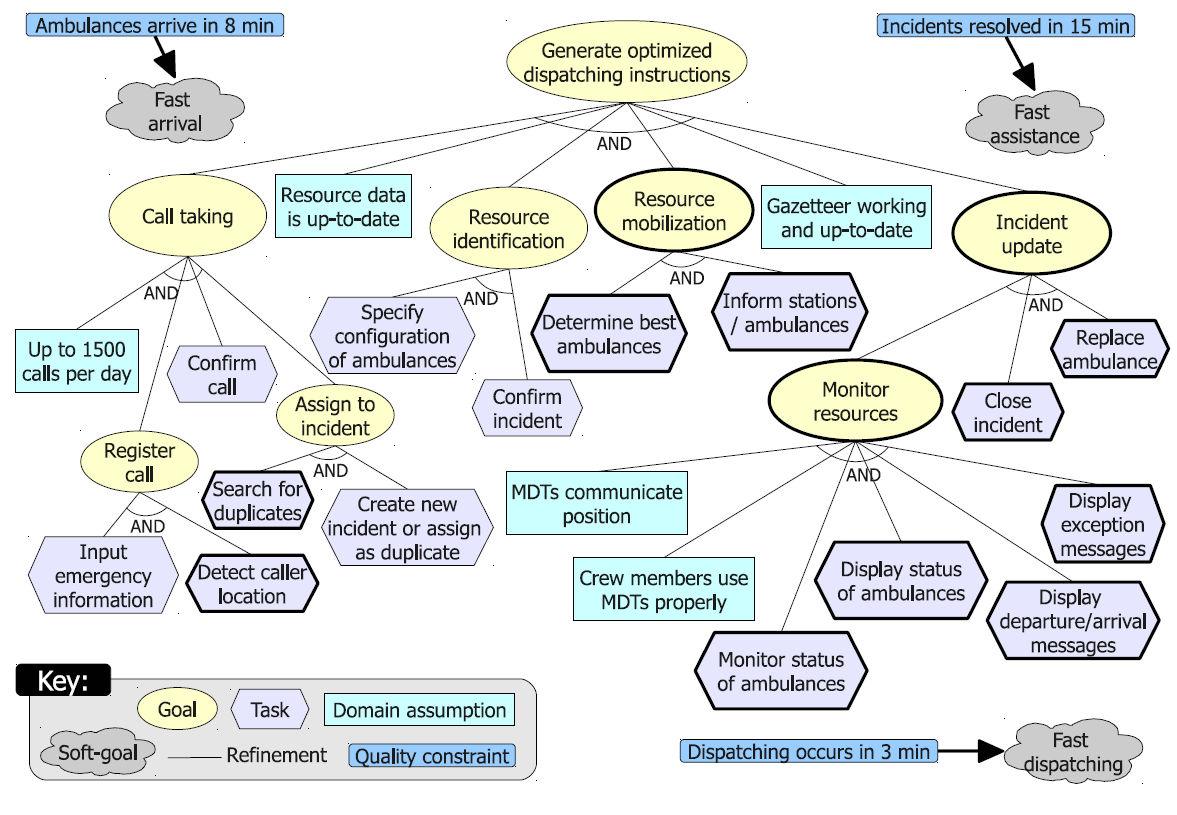
\includegraphics[width=1\textwidth]{figuras/modelos/ACAD-Simples.png}
	\caption{Exemplo de modelos de objetivos ~\cite{tesevitor}}
	\label{figura-acad-simples}
\end{figure}

% ======================================================================================================
% SUBSEÇÃO Modelos de Objetivos em Tempo de Execução
% ======================================================================================================

\subsection{Modelos de Objetivos em Tempo de Execução}
\label{sec-referencial-engenharia-objetivos-runtime}

% Sistemas adaptativos
Muitas vezes os requisitos de um \textit{software} precisam ser modificados durante o ciclo de execução do mesmo. Além disso, durante o processo de especificação as partes interessadas no sistema podem apresentar requisitos condicionais, ou seja, que assumem diferentes configurações dependendo da ocorrência de determinada situação~\cite{souza2012requirement}. Em outras palavras, há a necessidade de sistemas que possam se automonitorar e, caso necessário, se adaptarem para que seus objetivos continuem sendo satisfeitos~\cite{dalpiaz2013runtime}. Esse tipo de sistema geralmente é composto por duas partes principais: a primeira sendo o sistema em si, que executa uma tarefa para cumprir um objetivo desejado e a segunda sendo um sistema de monitoramento do primeiro, que envia ao primeiro sistema instruções de modificação de suas configurações para que seus objetivos continuem sendo atendidos~\cite{souza2013awareness}. 

O sistema de monitoramento é construído fundamentado na premissa de que todo sistema possui um ciclo de retroalimentação (\textit{(feedback loop)})~\cite{brun2009engineering}, e assim realizam o processo de adaptação com base nesse ciclo, aplicando controladores de \textit{feedback} que monitoram o comportamento do sistema e injetam estratégias de adaptação~\cite{souza2013awareness}. O módulo adaptador do sistema verifica, de acordo com as saídas do sistema alvo, se os objetivos internos a esse estão sendo atendidos e, para isso, necessita importar o modelo de objetivos~\cite{souza2013awareness} enriquecido de elementos que indicam os requisitos a serem observados e as estratégias de adaptação relativas.

Modelos de sistemas adaptativos incluem requisitos autoconscientes, ou seja, requisitos definidos em relação ao sucesso, falha ou qualidade de serviço de outros requisitos~\cite{souza2013awareness}. Assim, esses requisitos são considerados ``requisitos especiais'' já que sua operacionalização está relacionada a mudança de outros requisitos~\cite{souza2012requirement}. Ademais, o comportamento do sistema é caracterizado por eventos que ocorrem em tempo de execução e que estão diretamente ligados a instâncias de objetivos~\cite{dalpiaz2013runtime}. Assim, é importante observar que essa abordagem é considerada orientada a objetivos já que os requisitos mencionados são derivados do refinamento de objetivos elicitados para o sistema.

%Awreqs
Requisitos autoconscientes são divididos em dois tipos principais: Requisitos de Percepção (\textit{Awareness Requirements} ou \awreqs)~\cite{souza2013awareness} e Requisitos de Evolução (\textit{Evolution Requirements} ou \evoreqs)~\cite{souza2012requirement}. \awreqs são requisitos que referem-se ao estado de outros requisitos em tempo de execução, representando situações onde as partes interessadas desejam que o sistema se adapte~\cite{souza2012requirement}. Podem se referir a qualquer tipo de elemento, sejam objetivos, \sofgoals, tarefas e pressuposições de domínio. Além disso, indicam o quão critico um requisito pode ser ao descrever o grau de tolerância a falhas do mesmo~\cite{souza2012requirement}. Antes da execução de um sistema, os requisitos estão em estado ``Não Decidido'' (\textit{undecided}), e então pode assumir os estados ``Sucesso'' (\textit{Succeeded}), ``Falha'' (\textit{Failed}), e no caso de objetivos e tarefas, ``Cancelado'' (\textit{Canceled})~\cite{souza2013awareness}. É facilmente notável que o processo de elicitação de requisitos de percepção só acontece depois que o modelo de objetivos é levantado, e assim como o processo de construção de objetivos, \awreqs devem ser sistematicamente criados.

%Evoreqs
\evoreqs são requisitos que modificam o espaço de comportamento do sistema, permitindo que novas alternativas de requisitos sejam usadas, baseando-se em um conjunto pré-definido de etapas de evolução para os requisitos monitorados~\cite{souza2012requirement}. Isto é, \evoreqs são requisitos que especificam uma série de operações primárias em relação a outros requisitos diante de determinadas situações, dizendo ao sistema como adaptar-se~\cite{souza2012requirement}, como por exemplo, adicionar ou remover um objetivo, modificar o estado de um objetivo (em nível de instância), desfazer as ações de uma execução que resultou em falha, entre outras~\cite{souza2013requirements}.

Em suma, \awreqs especificam quando um determinado objetivo precisa de mudanças para continuar a ser atendido, enquanto \evoreqs especificam como executar tais mudanças. A seguir, o modelo de exemplo apresentado na seção~\ref{sec-referencial-engenharia-objetivos} é novamente apresentado, porém com novos requisitos de adaptação que são devidamente discutidos na próxima sessão.

% ======================================================================================================
% SUBSEÇÃO Exemplo de Caso de Uso
% ======================================================================================================
\subsection{Exemplo de Modelagem de Caso de Uso}
\label{sec-referencial-engenharia-objetivos-exemplo}

Na Figura~\ref{figura-acad-completo} é apresentado o modelo completo do sistema de despacho de ambulâncias (\textit{Adaptive Computer-aided Ambulance Dispatch} ou \textit{A-CAD}), nele observa-se o objetivo principal ``Gerar Instruções de Despacho Otimizadas'', representado por uma oval, que é imediatamente refinado em outros objetivos e em uma pressuposição de domínio (retângulo), o refinamento entre o objetivo raiz e seus filhos imediatos é do tipo ``E'' e portanto, para que o objetivo principal seja considerado satisfeito, todos as suas decomposições de primeiro grau precisam ser satisfeitas. Então, verifica-se que o primeiro nível de refinamento do objetivo principal é composto de:

\begin{itemize}
	\item Objetivo: ``Gerenciar Chamadas''
	\item Objetivo: ``Identificação de Recursos''
	\item Objetivo: ``Mobilização de Recursos''
	\item Objetivo: ``Obtenção de Mapas''
	\item Pressuposição de Domínio: ``Dados sobre recursos está sempre atualizado''
\end{itemize}

\begin{figure}[h]
	\centering
	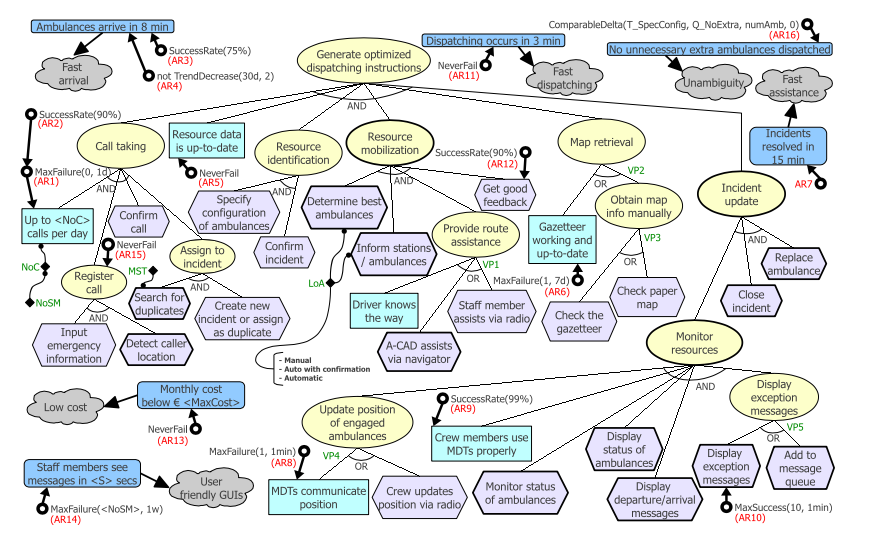
\includegraphics[width=1\textwidth]{figuras/modelos/ACAD-Completo.png}
	\caption{Exemplo de modelos de objetivos de um sistema de despacho de ambulâncias ~\cite{tesevitor}}
	\label{figura-acad-completo}
\end{figure}

O processo de refinamento do modelo então segue até que todos os objetivos sejam completamente refinados em tarefas ou pressuposições de domínio. \sofgoals são representados por nuvens e refinados em critérios de operacionalização representados por retângulos com cantos arredondados. Exemplificando, o \sofgoal ``Chegada Rápida''é operacionalizado por ``Ambulâncias chegam em oito minutos'', assim, tem-se um critério claro de satisfação para um objetivo que antes possuía diversos tipos de interpretação, porém agora, sabe-se que uma ambulância chega rapidamente se consegue estar no local do acidente em menos de oito minutos a partir da chamada.

Os requisitos de percepção são representados por um círculo oco. Por exemplo, o \awreq identificado por ``AR15'', indica que o objetivo ``Registrar Chamados'' deve ``Nunca falhar''. Os \evoreqs referentes a cada um dos \awreqs não são representados nesse modelo, e devem ser especificados em forma de sequencia de operações sobre os elementos do modelo de objetivos (essa escolha visa aprimorar a legibilidade do modelo). Além dos \awreqs, são especificados também os parâmetros de controle (\textit{control parameters}), representados por losangos, que indicam parâmetros do sistema que podem ser reconfigurados durante a adaptação. Todas as formas de representação estão resumidas na Figura~\ref{figura-elementos-gore-eca}.

\begin{figure}[h]
	\centering
	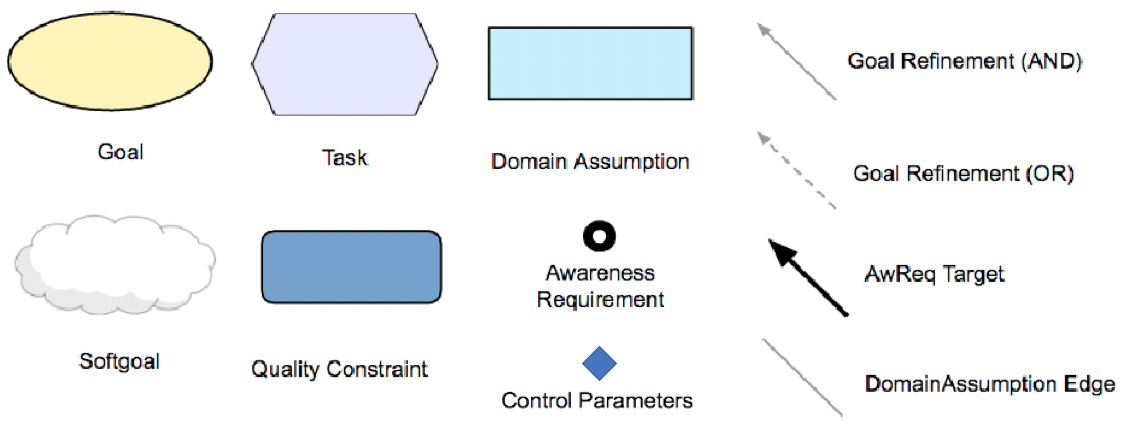
\includegraphics[width=1\textwidth]{figuras/modelos/Elementos-GORE.png}
	\caption{Representação gráfica de elementos de \gore}
	\label{figura-elementos-gore-eca}
\end{figure}

Sobre os \evoreqs do ``AR15'', podemos definir seus respectivos Requisitos de Evolução. Primeiramente, se o objetivo vir a falhar, define-se a primeira estratégia de adaptação como ``Tentar Novamente em 5 segundos no máximo uma vez'' (\texttt{RetryStrategy(5000)}), caso falhe mais do que uma vez, aplica-se outra estratégia ``Diminuir Condições ao Desabilitar Filho'' (\texttt{RelaxDisableChild(TDetectCaller)}), que desativa o requisito ``Detectar Localização da Ligação'', também aplicado no máximo uma vez. Essas decisões são sumarizadas na tabela \ref{tabela-evoreqs-ar15}.

\begin{table}[]
	\centering
	\caption{Tabela de especificação das estratégias de adaptação de AR15.}
	\label{tabela-evoreqs-ar15}
	\begin{tabular}{lll}
		AR15 & NeverFail(G\_RegCall) & \begin{tabular}[c]{@{}l@{}}1. Retry(5000)\\ 2. RelaxDisableChild(T DetectCaller)\end{tabular}
	\end{tabular}
\end{table}

O processo de especificação de como as estratégias de evolução são realizadas pelo sistema é discutido na próxima seção.

% ======================================================================================================
% SEÇÃO Zanshin
% ======================================================================================================

\section{Zanshin}
\label{sec-referencial-zanshin}

Apresentado por~\cite{tesevitor} e baseado em várias das premissas discutidas até aqui, \zanshin é um \textit{framework} que utiliza de ciclos de retro-alimentação para monitorar sistemas e enviar estratégias de adaptação com base em informações de modelos de requisitos orientados a objetivos enriquecidos com elementos como os \awreqs e os \evoreqs. O nome \zanshin vem de um termo usado em artes marciais japonesas e significa estado de completa consciência.

Em tempo de execução, os elementos do modelo de objetivos são representados por classes e instanciados cada vez que o usuário (ou sistema) busca atingir um objetivo, e então o sistema passa a enviar mensagens a essas instâncias quando detectar falhas. Percebe-se assim, que objetivos e pressuposições de domínio não são tratadas como invariantes que devem sempre ser atingidas, já que o sistema pode falhar ao tentar atingir seus objetivos iniciais, e assim o sistema de adaptação lidará com essas falhas e tomará medidas para que os objetivos voltem a ser satisfeitos~\cite{souza2013requirements}.

Assim como o monitoramento de objetivos através do \textit{Feddback Loop}, o \zanshin também monitora Parâmetros (\textit{Parameters}) que podem ser definidos em dois tipos. Primeiro, os Pontos de Variação (ou \textit{Variation Points}), que representam refinamentos do tipo ``OU'' (\textit{OR}). Por exemplo, o VP4 do modelo de objetivos do sistema A-CAD (Figura~\ref{figura-acad-completo}) que refere-se ao objetivo ``Atualizar posição de ambulâncias em uso'' especifica que atualizações de posição das ambulâncias podem ser obtidas automaticamente ou via rádio. Segundo, as Variáveis de Controle (ou \textit{Control Variables}), que são abstrações referentes a pontos de variação repetitivos ou usados em grande escala, como por exemplo a variável MST (``Tempo de Busca Mínimo'' ou \textit{Minimum Search Time}), que refere-se a tarefa ``Procurar por (incidentes) duplicados''.

O metamodelo dos modelos de objetivos usados no \zanshin é representado na Figura~\ref{figura-metamodelo-antigo}, e especificado no código do \textit{framework} como um modelo \emf e carregado em memória como objetos \java usando a API do \eclipse para \emf. Nessa caso, o modelo \emf representa os tipos de requisitos em nível de classe~\cite{souza2013requirements}. 

\begin{figure}[h]
	\centering
	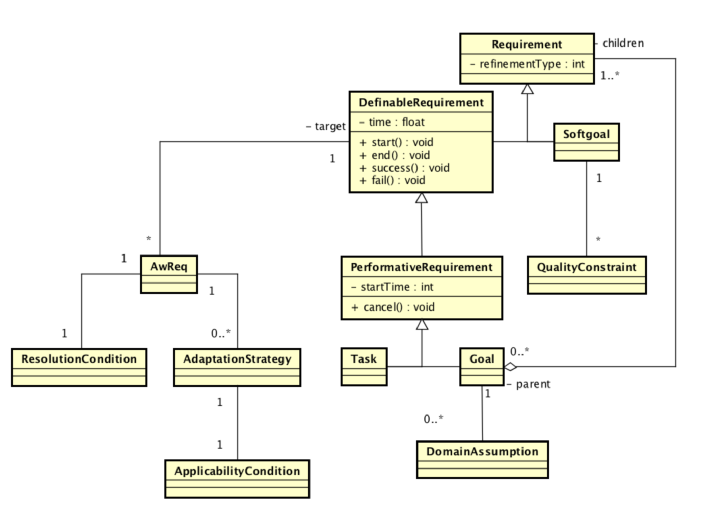
\includegraphics[width=1\textwidth]{figuras/metamodelos/metamodelo-zanshin-antigo.png}
	\caption{Metamodelo que define a sintaxe abstrata para o \zanshin}
	\label{figura-metamodelo-antigo}
\end{figure}

De uma maneira geral, o \zanshin é ser divido em quatro componentes. Essa seção discute dois módulos principais: o componente de monitoramento e o componente de adaptação.

% ======================================================================================================
% SUBSEÇÃO Zanshin: Monitoramento
% ======================================================================================================
\subsection{Monitoramento}
\label{sec-referencial-zanshin-monitoramento}

O módulo de monitoramento necessita que o sistema alvo implemente funcionalidades de registro (\textit{logs}). Através do registro, o sistema pode detectar mudanças nos estados das instâncias de um \awreq e assim notificar o serviço de adaptação sobre as mudanças ocorridas. 

Para identificar o modelo de objetivos do sistema alvo, o componente de monitoramento necessita da especificação do modelo do sistema também em \emf. Através dele, o \zanshin criará instancias desses objetivos extendendo as de classes carregadas do metamodelo de \gore referentes ao tipo de cada um deles. Ou seja, o modelo do sistema deve especificar objetos que extendam os disponíveis no metamodelo de \gore (Figura~\ref{figura-metamodelo-antigo}). Por exemplo, ao criar tarefa ``Especificar configuração de ambulâncias'', o sistema criará uma instancia dessa tarefa específica, que fará referência a classe \texttt{Task} criada no momento em que o metamodelo foi importado. A classe de tarefa especializa a classe \texttt{PerformativeRequirement} que é uma especialização \texttt{DefinableRequirement}. 

\textit{Performative Requirements} definem os tipos de requisitos que são ou podem ser refinados em tarefas, e assim possuem ações que são executadas pelo sistema ou seus usuários. Enquanto \textit{Definable Requirements} são os requisitos que deve possuir um estado definido em algum momento da execução, como por exemplo os objetivos e pressuposições de domínio.

Assim que o sistema cria as classes dos requisitos do sistema alvo, o processo de monitoramento apoia nos métodos definidos nas metaclasses \texttt{DefinableRequirement} e \texttt{PerformativeRequirement}~\cite{tesevitor} para realizar a monitoração, os métodos disponíveis são:
\begin{itemize}
	\item \texttt{start()}: esse método é chamado nas classes de critérios de qualidade e pressuposições de domínio imediatamente antes da análise de seu estado de satisfação. Para o caso de tarefas, esse método é chamado assim que um usuário inicia uma tarefa, e então todos os ancestrais a essa também tem esse método invocado.
	\item \texttt{sucess()}: chamado quando um requisito é satisfeito e propagado para todos os acentrais a esse objetivo para ``avisar'' que o filho chegou ao estado de sucesso.
	\item \texttt{fail()}: segue a mesma lógica dos item anteriores, propagando a ``falha'' de um requisito aos seus ancestrais.
	\item \texttt{cancel()}: para o caso de requisitos como objetivos e tarefas, esse método é usado quando um procedimento é cancelado pelo usuário, e usa da mesma lógica de propagação dos métodos anteriores para informar o ocorrido aos pais.
	\item \texttt{end()}: chamado assim que um requisito retorna dos estados de sucesso, falha ou cancelamento.
\end{itemize}

Através da descrição dos métodos acima mencionados, é possível entender como o processo de monitoramento funciona: basicamente os requisitos monitorados possuem métodos que podem ser chamados em cada caso que assumem, seja de sucesso, falha o ou cancelamento. Assim que chamados, os métodos invocam os mesmos métodos nos elementos pais, permitindo que a atualização de um requisito se propague a todos os elementos que interessem, atualizando assim todo o modelo.

Logo que o componente monitor detecta uma mudança de estado em um requisito, ou seja, assim que qualquer um dos métodos acima é invocado, ele imediatamente envia uma notificação sobre essa mudança ao módulo de adaptação, que então inicia o processo definido para aquele determinado requisito de percepção ~\cite{tesevitor}.

\subsection{Adaptação}
\label{sec-referencial-zanshin-adaptacao}
Em termos de implementação, o algoritmo do módulo de adaptação cria uma sessão para cada \awreq que está sendo monitorado e então gera uma fila de eventos que se referem a estratégias de adaptação. Assim, essa linha de eventos pode ser usada para verificar se uma estratégia é ou não aplicável a determinada situação. Primeiramente, deve-se verificar o estado de um objetivo apontado por um \awreq, para isso é checada a condição de resolução daquele. Então, caso uma avaliação considere que o objetivo está em estado de falha, o sistema segue (seguindo uma ordem pré-definida) a lista de estratégias de adaptação disponíveis, procurando alguma que tenha sua condição de aplicabilidade verdadeira. Caso encontre, aplica a estratégia de adaptação definida por aquela condição de aplicabilidade e então retorna ao estado inicial, onde a checagem da satisfabilidade do objetivo é realizada novamente. Caso o sistema retorne a fase de checagem do estado do objetivo e esse ainda não tenha sido satisfeito, o processo começa novamente. Caso não encontre uma condição para aplicar uma estratégia, o sistema ativa o método ``abortar'' (\texttt{abort()})~\cite{souza2013requirements}. 

Ao final, quando uma sessão de adaptação é considerada resolvida, a mesma deve ser terminada e se for necessário que o processo seja aplicado novamente, uma nova sessão é criada. Entretanto, se uma sessão termina sem ter resolvido o problema, o \textit{framework} continuará trabalhando nela do ponto em que parou assim que receber uma nova requisição para adaptação daquele mesmo \awreq. Porém, algumas estratégias também podem forçar que a sessão seja reiniciada quando executada ~\cite{souza2013requirements}. Essa processo é conhecido como Evento de Ação-Condição (\textit{Event Condition Action} ou \textit{ECA}) ~\cite{morin2009models}.

\subsubsection{ECA}
\label{sec-referencial-zanshin-eca}

O código a seguir resume o processo \textit{ECA} para realizar a seleção de estratégias de adaptação:

\begin{lstlisting}[caption={Código do processo ECA},label={listagem-estrategias-AR15}]
processEvent(ar : AwReq) {
	session = findOrCreateSession(ar.class);
	session.addEvent(ar);
	solved = ar.condition.evaluate(session);
	if(solved) break;

	ar.selectedStrategy = null;
	for each s in ar.strategies {
		appl = s.condition.evaluate(session);
		if (appl) {
			ar.selectedStrategy = s;
			break ;
		}
	}

	if (ar.selectedStrategy == null)
		ar.selectedStrategy = ABORT;

	ar.selectedStrategy.execute(session);
	ar.condition.evaluate(session);
}
\end{lstlisting}

O algoritmo incia obtendo a sessão de adaptação referente a classe do \awreq requisitado (caso não haja uma sessão, uma nova é criada). Obtida a sessão de adaptação, o algoritmo tem então acesso a lista de eventos de aplicabilidade referentes, então, adiciona o \awreq a sessão e imediatamente verifica o estado da mesma (verificando a condição de resolução), parando caso tenha retornado estado de sucesso. Caso contrário, o processo continua procuando por uma estratégia que seja aplicável, verificando se a condição de aplicabilidade é verdadeira. Caso for verdadeira, interrompe o processo e dá a sessão de adaptação uma nova chance de verificar o estado do \awreq. Caso todas as condições sejam falsas e nenhuma estratégia seja selecionada, seleciona a estratégia padrão (\texttt{abort()}) e termina o processo~\cite{tesevitor}. 

Para exemplificar esse processo, tomemos novamente o \awreq ``AR15'', que garante que o requisito ``Registrar chamada'' deve nunca falhar. Caso seja detectado pelo processo de monitoramento que esse requisito apresenta estado de falha, o módulo monitor imediatamente ativa o módulo de adaptação, que segue o processo ECA para aplicar estratégias ao ``AR15''. Pela Listagem~\ref{listagem-estrategias-AR15}, ve-se que a condição de resolução desse requisito é do tipo \texttt{SimpleResolutionCondition} e que a primeira estratégia a ser selecionada é \texttt{RetryStrategy}, ou seja, tentar novamente (em 5s), entretanto, essa estratégia possui a condição de aplicabilidade \texttt{MaxExecutionsPerSessionApplicabilityCondition}, o que significa que ela só pode ser aplicada uma vez naquela sessão. Caso essa condição seja falsa, a próxima estratégia refere-se a desativar um dos filhos desse objetivo (\texttt{RelaxDisableChildStrategy}), no caso a tarefa ``Detectar localização da chamada'', e possui a mesma condição de aplicabilidade. Se nenhuma dessas condições puder ser satisfeitas, então o sistema aborta, caso contrário, seleciona a primeira estratégia aplicável e verifica novamente o estado do objetivo. A condição \texttt{SimpleResolutionCondition} refere-se ao fato de que um objetivo é dito satisfeito apenas se seus filhos estiverem em estado de sucesso (respeitando a regra booleana do refinamento). 

\begin{lstlisting}[caption={Estratégias de adaptação de AR15},label={listagem-estrategias-AR15}]
<awreqs xsi:type="acad:AR15">										
	<condition xsi:type="eca:SimpleResolutionCondition"/>
		<strategies xsi:type="eca:RetryStrategy" time="5000">
			<condition xsi:type="eca:MaxExecutionsPerSessionApplicabilityCondition" maxExecutions="1"/>
		</strategies>
		<strategies xsi:type="eca:RelaxDisableChildStrategy" child="//@rootGoal/@refinements.0/@refinements.0/@refinements.1">
			<condition xsi:type="eca:MaxExecutionsPerSessionApplicabilityCondition" maxExecutions="1"/>
		</strategies>
</awreqs>
\end{lstlisting}

É importante salientar que as classes referentes a estratégias de adaptação, assim como as condições de aplicabilidade e resolução podem ser extendidas para casos mais complexos, envolvendo inclusive a interação humana ~\cite{tesevitor}.

%For example, the trivial case is considering the problem solved if the (next) AwReq evaluates to success, but this abstract class can be extended to provide di↵erent kinds of resolution conditions, including, e.g., involving a human-in-the-loop to confirm if the problem has indeed been solved, organizing conditions into AND/OR-refinement trees (like in a goal model), etc.

% ======================================================================================================
% SUBSEÇÃO DESENVOLVIMENTO ORIENTADO A MODELOS
% ======================================================================================================
\section{Desenvolvimento Orientado a Modelos}
\label{referencial-mdd}
Pesquisadores vem tentando ao longo dos anos criar abstrações que ajudem programadores a focar no conteúdo do desenvolvimento ao invés das especifidades da tecnologia de criação adotada~\cite{viyovic2014sirius}. O Desenvolvimento Orientado a Modelos  pode ser visto como a forma de programação de mais alto nível de abstração existente atualmente~\cite{atkinson2003model}, promovendo o uso de artefatos do processo de desenvolvimento de software para lidar com complexidade através de abstração~\cite{viyovic2014sirius}. Em outras palavras, MDD parte da premissa que um sistema é um modelo consistente com seu metamodelo~\cite{vujovic2014comparative}, assim, em vez de exigir que programadores escrevam cada simples detalhe da implementação de um sistema, permite que uma funcionalidade necessária para um software pode ser visualmente modelada ~\cite{atkinson2003model}. Sendo assim, essa técnica viabiliza que muitas atividades complexas (porém rotineiras) sejam automatizadas na área de programação de software, como por exemplo o suporte a persistência, interoperabilidade e distribuição ~\cite{atkinson2003model}.

A modelagem usa da percepção visual humana para melhorar o processo de compreensão sobre o domínio de um software, já que modelos nos auxiliam a entender problema complexos e suas possíveis soluções através da abstração. Assim, MDD baseia-se na premissa de que o desenvolvimento de software deve focar principalmente na produção de modelos e não na criação de código ~\cite{selic2003pragmatics}. A primeira vantagem dessa abordagem é que podemos usar conceitos mais ligados ao domínio do problema que software vai resolver do que conceitos técnicos ligados a linguagem de programação. Essa vantagem acarreta em alguns outros benefícios: modelos são mais compreensíveis do que códigos e portanto, tornam-se também mais fáceis de especificar e manter~\cite{selic2003pragmatics}. Além disso, modelos são menos sensíveis a alterações de tecnologias, ou seja, são independentes de plataforma~\cite{selic2003pragmatics}. Em conclusão, observa-se que o principal (porém não único) aspecto de MDD é a produção automática de código através da interpretação de modelos visuais~\cite{selic2003pragmatics, viyovic2014sirius}.

\subsection{Eclipse Modeling Framework}
O \eclipse é um projeto de código aberto com o objetivo de prover uma plataforma de desenvolvimento altamente integrada. O processo de criação de sistemas no \eclipse pode ser divido em alguns projetos, entre eles o Projeto de Modelagem (\textit{Modeling Project}), que foca em tecnologias baseadas no desenvolvimento orientado a modelos~\cite{steinberg2008emf}. Esse ambiente é chamado de \textit{Eclipse Modeling Framework} ou \textit{EMF}, e provê funcionalidades como transformação de modelos, integração de bases de dados e geração de editores gráficos~\cite{steinberg2008emf}. Modelos especificados através de \emf relacionam conceitos de modelagem diretamente a seus conceitos de implementação, sendo a união das tecnologias \uml, \xml e \java, permitindo a conversão automática entre todas essas ferramentas~\cite{steinberg2008emf}. 

A tecnologia \emf pode ser melhor explicado com um exemplo: um sistema de gerenciamento de ordem de compras de uma loja, que necessite incluir casos como ``cobrar'' e ``entregar'' em um endereço, e uma coleção de itens (nesse caso compras). A figura~\ref{exemplo-uml} mostra o diagrama em \uml do sistema. Esse modelo pode também ser descrito dentro do \emf usando modelos \ecore, como na Figura~\ref{exemplo-ecore}. Modelos \ecore são basedos no metamodelo para especificação exibido na Figura~\ref{metamodelo-ecore}, onde classes são representadas por \texttt{EClass}, atributos por \texttt{EAttribute}, relações por \texttt{EReference} e tipos de dados por \texttt{EDataType}. Assim, a ``conversão'' do modelo \uml para \ecore é dada ao se instanciar classes de \ecore de acordo com a especificidade do domínio do problema, como pode ser visto na Figura~\ref{exemplo-uml-to-ecore}~\cite{steinberg2008emf}. 

\begin{figure}[h]
	\centering
	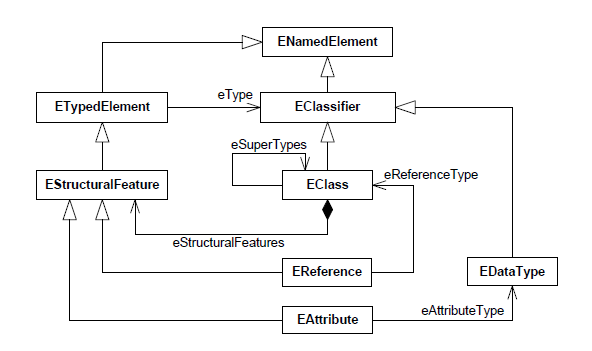
\includegraphics[width=0.95\textwidth]{figuras/exemplos-emf/metamodelo-ecore.png}
	\caption{Metamodelo de \ecore~\cite{kern2008interchange}}
	\label{metamodelo-ecore}
\end{figure}

\begin{figure}[h]
	\centering
	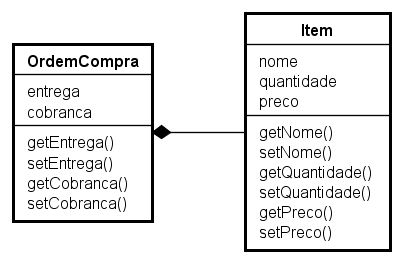
\includegraphics[width=0.65\textwidth]{figuras/exemplos-emf/exemplo-uml.png}
	\caption{Classes do diagrama do exemplo em \uml}
	\label{exemplo-uml}
\end{figure}

\begin{figure}[h]
	\centering
	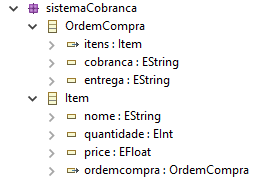
\includegraphics[width=0.7\textwidth]{figuras/exemplos-emf/exemplo-ecore.PNG}
	\caption{Classes do diagrama do exemplo em \ecore}
	\label{exemplo-ecore}
\end{figure}

Assim que o modelo é detalhado em \ecore, o \emf está pronto para gerar código automaticamente, seguindo os seguintes passos:

\begin{itemize}
	\item Para cada tipo \texttt{EClass} são criadas uma interface e a classe de implementação correspondente. Então para o exemplo de classe \texttt{OrdemCompra} serão criadas a interface \texttt{OrdemCompra} e a classe \texttt{OrdemCompraImpl}. Essa especificação permite que sejam implementadas funções de persistência e distribuição, porém não serão discutidas aqui por fugirem do escopo desse trabalho.
	\item As classes do tipo \texttt{EAtributte} são transformadas em atributos nas classes correspondentes
	\item As classes tipo \texttt{EReference} são transformadas em referências nas respectivas classes as quais referenciam.
\end{itemize}

\begin{figure}[h]
	\centering
	
\includegraphics[width=1\textwidth]{figuras/exemplos-emf/uml-to-ecore.png}
	\caption{Conversão do diagrama de exemplo de \uml para \ecore}
	\label{exemplo-uml-to-ecore}
\end{figure}

Em suma, o \framework de modelagem do \eclipse permite que usuários criem modelos apoiados em metamodelos, e baseando-se no modelo criado, gerem partes de código de sistema~\cite{vujovic2014comparative}.

%https://books.google.com.br/books?id=sA0zOZuDXhgC&lpg=PT23&ots=2IQIWZWqNm&dq=eclipse&lr&hl=pt-BR&pg=PT45#v=onepage&q=eclipse&f=false

\subsection{Sirius}

O \sirius é um plugin que simplifica o \framework de Modelagem Gráfica (\textit{Graphical Modeling Framework} ou \textit{GMF}) do \eclipse, reduzindo a complexidade de uso do mesmo e permitindo a produção de editores gráficos de modelos personalizados~\cite{viyovic2014sirius}. O \sirius é construído em cima do fato de que o \eclipse provê utilidades para (des)serialização de modelos, checagem de condições e geração de editores baseados em \emf~\cite{budinsky2004eclipse}. Representações criadas com \sirius podem ser apresentadas em diagramas, tabelas e árvores~\cite{viyovic2014sirius}. Em síntese, \sirius provê ferramentas que permitem a especificação de um modelo de um domínio qualquer em diferentes perspectivas~\cite{vujovic2014comparative}.

Através de modelos de especificação (\textit{Viewpoint Specification Model} ou VSM), o \textit{plugin} permite especificar a estrutura, aparência e comportamento do metamodelo do editor a ser criado~\cite{viyovic2014sirius}. Os VSMs são especificados através de arquivos \textit{.odesign}~\cite{viyovic2014sirius}, e baseam-se na especificação do metamodelo em \ecore. Um exemplo de caracterização de representação de modelos é mostrado na figura~\ref{exemplo-sirius} retirada de~\cite{viyovic2014sirius}.

\begin{figure}[h]
	\centering
	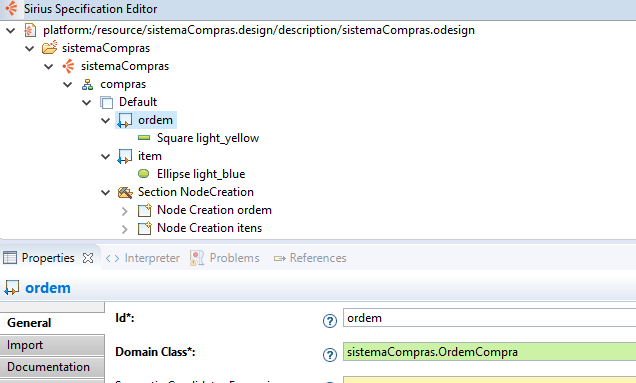
\includegraphics[width=0.9\textwidth]{figuras/exemplos-emf/exemplo-sirius-vsm.png}
	\caption{Exemplo de \textit{Viewpoint Specification Model}}
	\label{exemplo-sirius}
\end{figure}

\sirius provê vários mecanismos que auxiliam no gerenciamento da complexidade de modelos~\cite{madiot2015eclipse}:

\begin{itemize}
	\item \textbf{Camadas}: é possível separar elementos em camadas diferentes, e ativar ou desativar essas.
	\item \textbf{Filtros}: exibir ou esconder elementos dependendo de determinada condição.
	\item \textbf{Fersonalização de Estilos}: permite modificar propriedades gráficas de elementos do diagrama.
	\item \textbf{Regras de Validação}: permite que a qualidade do modelo seja avaliada.
\end{itemize}


% ==============================================================================
% TCC - César Henrique Bernabé
% Capítulo 3 - Zanshin
% ==============================================================================

\chapter{Zanshin}
\label{sec-zanshin}

Esta seção trata do processo de reavaliação do metamodelo operacional do sistema \zanshin, anteriormente já apresentado na Figura~\ref{figura-metamodelo-antigo}.

% ======================================================================================================
% SUBSEÇÃO Motivação
% ======================================================================================================
\section{Motivação}
\label{sec-zanshin-motivacao}
Durante estudos realizados sobre a implementação do \framework \zanshin, foram detectadas algumas oportunidades de melhoria relacionadas principalmente ao metamodelo de objetivos utilizado pelo sistema. A maioria das adequações identificadas referem-se a dois motivos: ou o metamodelo não era restrito o suficiente, deixando que algumas situações indesejadas pudessem ser modeladas; ou o metamodelo não refletia mais alguns conceitos de \gore que foram melhores elaborados em discussões sobre o tema. 

% ======================================================================================================
% SUBSEÇÃO Revisão do Metamodelo
% ======================================================================================================
\section{Revisão do Metamodelo}
\label{sec-zanshin-revisao}
Uma análise de cada elemento do metamodelo antigo é feita a seguir:

\begin{enumerate}
	%1
	\item \textbf{Requirement}: o fato desse elemento estar no topo da hierarquia e todos os outros elementos serem especializações dele faz com que suas características sejam herdadas por todos os outros componentes do modelo. Porém, nota-se que algumas características na verdade são inerentes a apenas alguns elementos. Por exemplo: \textit{Requirement} possui a relação de agregação \textit{Parent} para \textit{Children}, permitindo que cada elemento tenha zero ou um ``Pai'' e um ou vários ``Filhos''. Entretanto, a agregação pai/filho é indesejada nos elementos \awreq, \textit{DomainAssumption} e \textit{QualityConstraint}, visto que esses não são refinados, apenas possuem ``alvos''. \label{p1}
	
	%2
	\item \textbf{DeinableRequirement} e \textbf{Softgoal}: \sofgoal possui o mesmo tipo de comportamento de um \textit{DefinableRequirement} e portanto, seria esperado que aquele também fosse uma especialização deste. Assim, com essa modificação seria desnecessário a utilização de duas classes (\textit{Requirement} e \textit{DefinableRequirement}) na composição do modelo, que poderiam perfeitamente ser reduzidas a apenas uma. \label{p2}
	
	%3
	\item \textbf{Softgoal} e \textbf{QualityConstraint}: O modelo permite que um \textit{Softgoal} contenha nenhuma operacionalização, o que não faria sentido pois assim não seria possível identificar quando esse elemento foi bem sucedido ou não. \label{p3}
	
	%4
	\item \textbf{DefinableRequirement} e \textbf{AwReq}: de acordo com as propostas apresentadas na literatura atual para os \awreqs (fontes?), fica claro que esses elementos, ao se referirem a qualquer outro tipo de elemento e tratarem especificamente do elemento ao qual se referem, deveriam ter na verdade uma relação de composição com o elemento mais alto da hierarquia de especializações, permitindo então que todos os outros elementos do modelo contivessem \awreqs. \label{p4}
	
	%5
	\item \textbf{Goal} e \textbf{Task}: \textit{Tasks} são refinamentos de \textit{Goal} e por isso seria importante que houvesse algum tipo de relacão direta entre os dois elementos, onde fosse possível identificar que quando um objetivo fosse operacionalizado por tarefas e quais seriam essas tarefas. Além disso, identificou-se uma oportunidade de melhoria da nomenclatura de ``\textit{Goal}'' para ``\textit{HardGoal}'', refletindo uma melhor impressão sobre o papel do elemento e as diferenças entre ambos. \label{p5}
	
	%6
	\item \textbf{DomainAssumption}: a forma como \textit{DomainAssumptions} se relacionam com os outros elementos poderia ser refinada, o objetivo aqui é que qualquer tipo de elemento que for passível de ser operacionalizado (\textit{PerformativeRequirement}) pudesse conter uma lista de referências a pressuposições de domínio. \label{p6}
\end{enumerate}

% ======================================================================================================
% SUBSEÇÃO Proposta
% ======================================================================================================
\section{Proposta}
\label{sec-zanshin-proposta}

Após levantamento das melhorias possíveis, foi elaborado o metamodelo apresentado na Figura~\ref{figura-metamodelo-novo}. 

\begin{figure}[h]
	\centering
	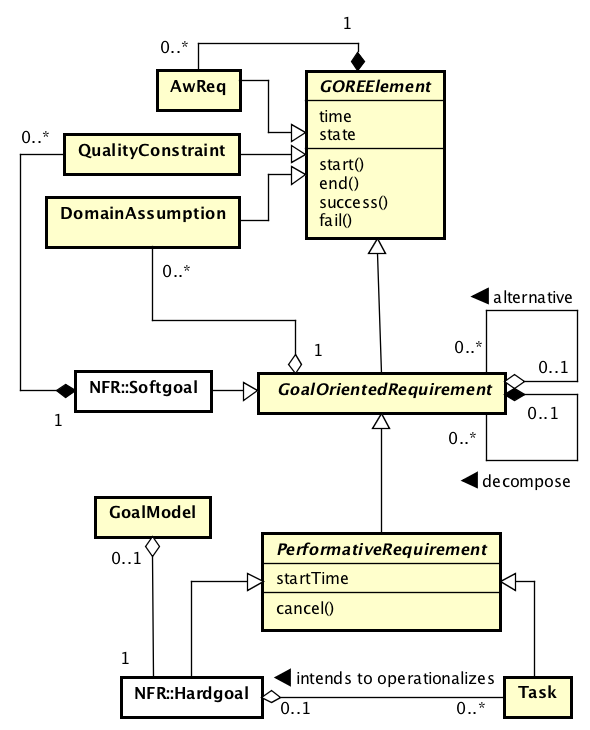
\includegraphics[width=0.7\textwidth]{figuras/metamodelos/metamodelo-zanshin-novo.png}
	\caption{Proposta de evolução do metamodelo do \framework \zanshin}
	\label{figura-metamodelo-novo}
\end{figure}

Primeiramente, pode-se observar que o as especialiações e relações de agregação e composição entre os elementos foram refinadas, assim, identifica-se que:

\begin{itemize}
	\item A partir de agora, todos os elementos são especializações de \textit{GOREElement}, que passa a englobar características das antigas classes \textit{Requirement} e \textit{DefinableRequirement}, resolvendo então parte do problema~\ref{p2}. 

	\item A agregação pai/filho agora ocorre em dois tipos e acontece em um elemento mais específico: um requisito pode ser decomposto (\textit{decompose}) em outros, referindo-se assim a refinamentos do tipo ``E'', ou refinado através da agregação denominada ``alternative'', que trata de alternativas a um requisito, ou seja, refinamentos do tipo ``OU''. Dessa forma o metamodelo pode retratar melhor os tipos de refinamentos admitidos e quais são, exatamente, os componentes que  os aceitam. Além do mais, a partir desta melhoria os refinamentos acontecem somente nos elementos que especializam \textit{GoalOrientedRequirement}, ou seja, somente \textit{Hardgoals}, \textit{Softgoal} e \textit{Tasks}. Essa modificação soluciona o problema~\ref{p1}.

	\item Nessa nova proposta, há uma relação de decomposição entre o elemento raiz (\textit{GOREElement}) e \awreq, portanto, explicita-se a noção de que qualquer requisito pode conter requisitos adaptativos, eliminando a outra parte do problema~\ref{p2}. Isso também tem um efeito positivo em relação a especificação do \xml usado para criar modelos específicos de domínio, que fica mais claro e conciso.
	
	\item \textit{Softgoal} e \textit{QualityConstraint} passam a se relacionar por meio de relação de decomposição, e portanto também fica mais evidente que todo \textit{Softgoal} deve ser operacionalizado por pelo menos um \textit{QualityConstraint}, dando fim assim ao problema~\ref{p3}.
	
	\item Nessa proposta, \awreqs tem uma relação direta de composição com o \textit{GOREElement} logo, define-se que qualquer tipo de requisito no modelo pode conter elementos de adaptação, assim resolve-se o problema~\ref{p4}.
	
	\item No novo metamodelo, foi criada uma relação direta entre \textit{Tasks} e \textit{Hardgoals} (denominados anteriormente por \textit{Goals}), assim fica explícito o relacionamento entre esses dois elementos, sinalizando que objetivos são refinados em tarefas, que podem ser refinadas apenas nelas mesmas. Soluciona-se então o problema~\ref{p5}.
	
	\item Propõe-se, por fim, uma relação de agregação entre \textit{DomainAssumption} e \textit{GoalOrientedRequirement}, assim fica claro que \textit{Domain Assumptions} são elementos que interagem apenas com \textit{Hardgoals}, \textit{Softgoals} e \textit{Tasks}, findando o problema~\ref{p6}.
	
\end{itemize}

Uma observação importante que deve ser feita refere-se ao fato de que um elemento só pode conter refinamentos exclusivamente do tipo ``E'' (``AND'') ou exclusivamente do tipo ``OR''. Essa decisão tem por objetivo facilitar a leitura e interpretação do diagrama, e não compromete a representatividade do modelo pois assume-se que caso necessário, o modelador pode agrupar refinamentos do mesmo tipo em um objetivo, como exemplificado na Figura~\ref{figura-refinamentos}.

\begin{figure}[h]
	\centering
	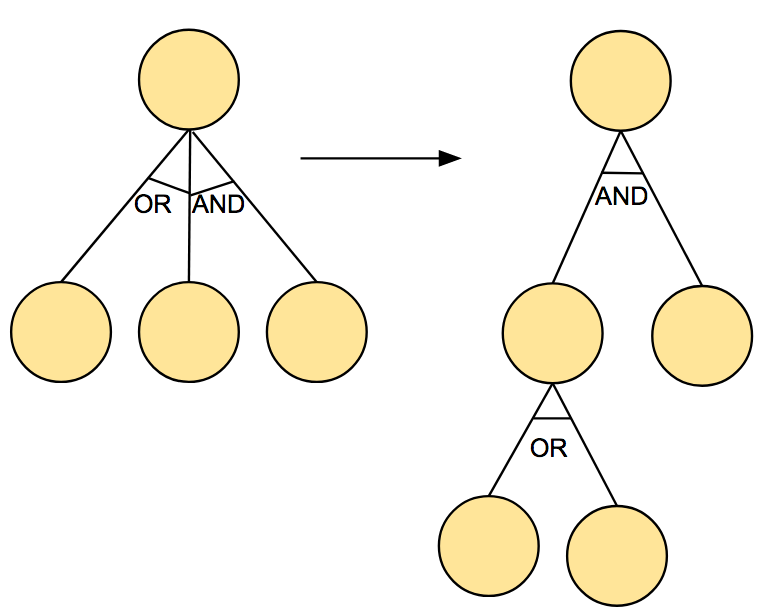
\includegraphics[width=0.7\textwidth]{figuras/metamodelos/exemplo-or-and.png}
	\caption{Exemplificação da representação de refinamentos no novo metamodelo.}
	\label{figura-refinamentos}
\end{figure}
% ==============================================================================
% TCC - César Henrique Bernabé
% Capítulo 4 - Unagi
% ==============================================================================
\chapter{Unagi}
\label{sec-unagi}

O editor gráfico \unagi foi desenvolvido com o principal objetivo de facilitar a criação de arquivos de especificação do modelo de dominio para uso no \zanshin, considerando que até então não havia nenhuma ferramenta que automatizasse esse processo, assim o usuário precisava escrever o arquivo \xml e \ecore manualmente. 

Usando um ferramental disponível na plataforma \eclipse para criação de editores gráficos usando \emf, além da utilização de aspectos de desenvolvimento dirigido por modelos, o processo de desenvolvimento do \unagi pode ser dividido em duas fases: a criação do editor gráfico usando \sirius e o desenvolvimento do conversor de diagramas apoiado em código gerado automaticamente por técnicas MDD (\mdd).

\vitor{Mencionar subseções.}

% ======================================================================================================
% SEÇÃO criação do Editor Gráfico
% ======================================================================================================
\section{Criação do Editor Gráfico}
\label{sec-unagi-criacao-editor}

A primeira parte do desenvolvimento da ferramenta consitiu  na criação do editor gráfico para modelagem de diagramas de objetivos para sistemas de adaptativos. Devido ao fato de \zanshin ser um sistema que também se baseia nas ferramentas da plataforma \eclipse, aliado ao fato dessa plataforma também prover todos os utensílios necessários para o desenvolvimento de editores de diagramas, como \ecore, \emf e o plugin \sirius, foi fácil decidir que para o desenvolvimento do \unagi também seriam usados os mesmos recursos, com objetivo assim de permitir maior compatibilidade com o \zanshin em trabalhos futuros.

Inicialmente, o mesmo modelo \ecore usado para operacionalização dos requisitos no \zanshin foi usado para geração automática de código dentro do \eclipse \emf. É importante salientar que junto com as classes específicas de domínio, o \emf também gera código automático para criação de editores e para criação de processos de teste e validação (Figura~\ref{figura-gera-codigo}). Assim, após completa especificação do \ecore, foi gerado código automático para implantação do editor. O código gerado pode então ser executado como uma aplicação \eclipse e a partir daí pode-se criar um editor de modelos personalizado usando o \sirius.

\vitor{Não fica claro no parágrafo acima que o editor que é gerado automaticamente não permite a criação do modelo de forma diagramática. Fica parecendo que o EMF gerou o Unagi com apenas um clique...}

\begin{figure}
	\centering
	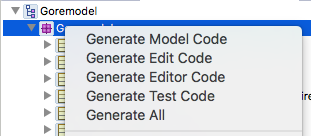
\includegraphics[width=0.5\textwidth]{figuras/unagi/exemplo-gera-codigo.png}
	\caption{Geração automática de código no \eclipse.}
	\label{figura-gera-codigo}
\end{figure}

Rodando na instância do \eclipse a partir do código de editor gerado automaticamente, o plugin \sirius permite que sejam definidos pontos de perspectiva com diferentes especificações de representação gráfica para os objetos do modelo \ecore. Essa especificação é realizada a partir da criação de Projetos de Especificação de Perspectiva (\textit{Viewpoint Specification Project} ou \textit{VSP}), onde são definidos como os elementos serão representados, como suas instâncias serão armazenadas nas classes do metamodelo \ecore, qual o comportamento do modelo quando relações são criadas, dentre outros.

A princípio, é criado dentro do modelo de VSP uma camada (\textit{layer}) que representa a perspectiva a ser representada, nelas são especificados os elementos do modelo \ecore que serão representados, aqui chamados de \textit{Nodes}, que pode ter um estilo padrão ou um estilo condicionado a determinada situação, além disso, pode-se usar formas geométricas predefinidas ou importar imagens externas. 

Como visto na Figura~\ref{exemplo-sirius-vsp}, o elemento \textit{Goal} tem como representação padrão uma elipse amarela. Essa representação pode ser mais bem configurada por meio da paleta de propriedades da mesma (Figura~\ref{figura-propriedades-personalizacao}), onde podem ser especificadas características visuais como cor da linha e tamanho do nome.

\begin{figure}
	\centering
	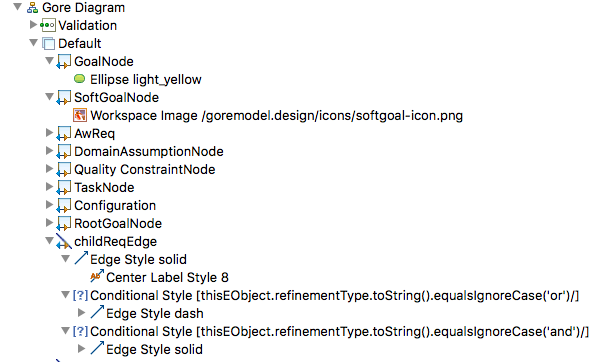
\includegraphics[width=1\textwidth]{figuras/unagi/exemplo-sirius-vsp.png}
	\caption{Sirius Viewpoint Specification Project.}
	\label{exemplo-sirius-vsp}
\end{figure}

\begin{figure}
	\centering
	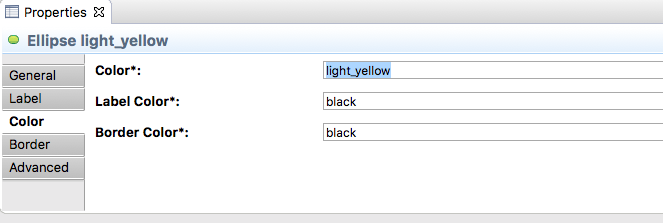
\includegraphics[width=1\textwidth]{figuras/unagi/exemplo-propriedades-personalizacao.png}
	\caption{Propriedades de Representação de Elemento em \sirius.}
	\label{figura-propriedades-personalizacao}
\end{figure}

Na Figura~\ref{exemplo-sirius-vsp} também pode-se observar que além da representação dos \textit{Nodes}, é necessário configurar a criação das linhas de ligação entre os elementos, pois por meio dessas são definidos os refinamentos entre os componentes do modelo. Em \texttt{childReqEdge} é especificado que se um objeto possui tipo de refinamento ``OU'' (``OR''), deve ser usado o tipo de linha tracejada, entretanto, se for do tipo ``E'' (``AND''), usa-se linha contínua. A linguagem usada para escrita de termos condicionais é conhecida como Acceleo Query Language~\cite{musset2006acceleo}, e será posteriormente discuta nesse capítulo.

Além da caracterização dos elementos que serão representados em uma perspectiva, o \sirius também necessita que sejam configuradas propriedades de instanciação dos elementos, assim, além dos \textit{Nodes} de represntação, devem ser criados os \textit{Nodes} de criação, mostrados na Figura~\ref{figura-criacao-node}, onde podem ser observados, por exemplo, a criação do \textit{Node Goal}. Nessa etapa é necessario que primeiramente seja especificado em que tipo de instância do metamodelo o novo objeto será armazenado, para o \textit{Node} de exemplo pode-se observar que há duas ocasiões:
\begin{itemize}
	\item Caso o elemento for o elemento pai, ou seja, a raiz da árvore de representação, deve ser armazenado em uma variável especial da classe \textit{GoalModel}, de nome \textit{rootGoal}. Esse caso é verificado ao checar se a variável ainda não foi definda (\texttt{Case[oclIsUndefined(container.rootGoal)]}).
	\item Caso o elemento for refinamento de qualquer nível do elemento pai, então é guardado na variável \textit{children} da classe \textit{GoalModel}.
\end{itemize}

Decididos os casos, é necessário criar uma instancia da classe relativa ao novo elemento, esse processo é definido por meio das propriedades da opção \textit{Create Instance} (Figura~\ref{figura-criacao-node}). Essas propriedades são definidas de acordo com o modelo \ecore, como pode ser visto na Figura~\ref{figura-propriedades-create-instance}. O campo \textit{referenceName} deve se referir a variável da classe de contenimento que será usada para armazenar o novo elemento, enquanto \textit{Type Name} refere-se à classe do novo componente do modelo.

\begin{figure}
	\centering
	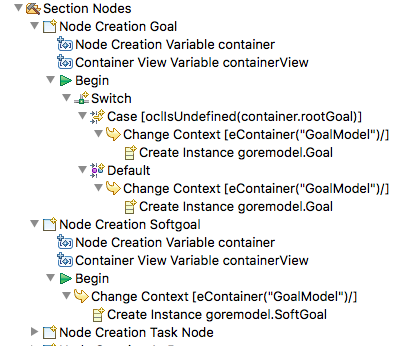
\includegraphics[width=0.7\textwidth]{figuras/unagi/exemplo-criacao-nodes.png}
	\caption{Criação de Nodes no \sirius - Exemplo de criação de nó.}
	\label{figura-criacao-node}
\end{figure}

\begin{figure}
	\centering
	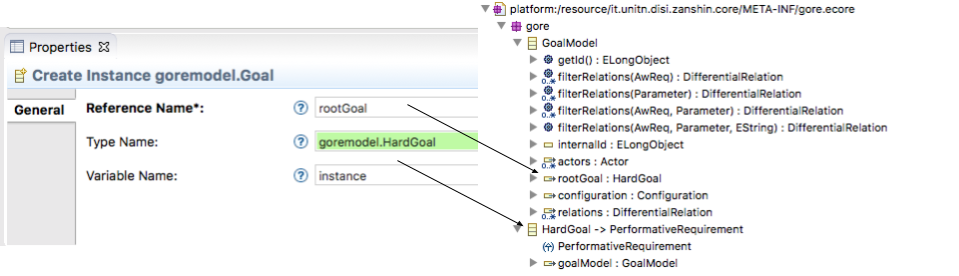
\includegraphics[width=1\textwidth]{figuras/unagi/exemplo-propriedades-create-instance.png}
	\caption{Criação de Nodes no \sirius - Exemplo de criação de instancia de nó.}
	\label{figura-propriedades-create-instance}
\end{figure}

Por fim, foi modelada uma perspectiva diferente para especificação das estratégias de adaptação dos \awreqs, permitindo que cada um tenha sua propria representação em um diagrama separado, com o objetivo de evitar que o modelo principal ficasse ``poluído'' por excesso de informação. 

% ======================================================================================================
% SUBSEÇÃO O Editor Gráfico
% ======================================================================================================
\subsection{O Editor Gráfico}
\label{sec-unagi-apresentacao-editor}

Após todo o processo de detalhamento da representação dos elementos do editor, é possivel então criar um modelo de especificação de perspectiva (\textit{Viewpoint Specification Model}), que permite a criação do diagrama usando recursos de arrastar e soltar, considerados intuitivos por estarem presentes na maioria dos editores gráficos atuais. A Figura~\ref{figura-paleta-unagi} mostra o editor em execução, onde pode ser vista a área de modelagem, bem como a paleta de elementos que podem ser criados, também é mostrada a paleta com tipos de refinamentos disponíveis para modelagem. Esses refinamentos podem ser selecionados e então desenhados apenas clicando no elemento de origem e destino, nesta ordem. As propriedades relativas a cada elemento do modelo podem ser modificadas por meio da paleta de opções que aparece na área inferior do editor (Figura~\ref{unagi-paleta-opcoes}).

\begin{figure}
	\centering
	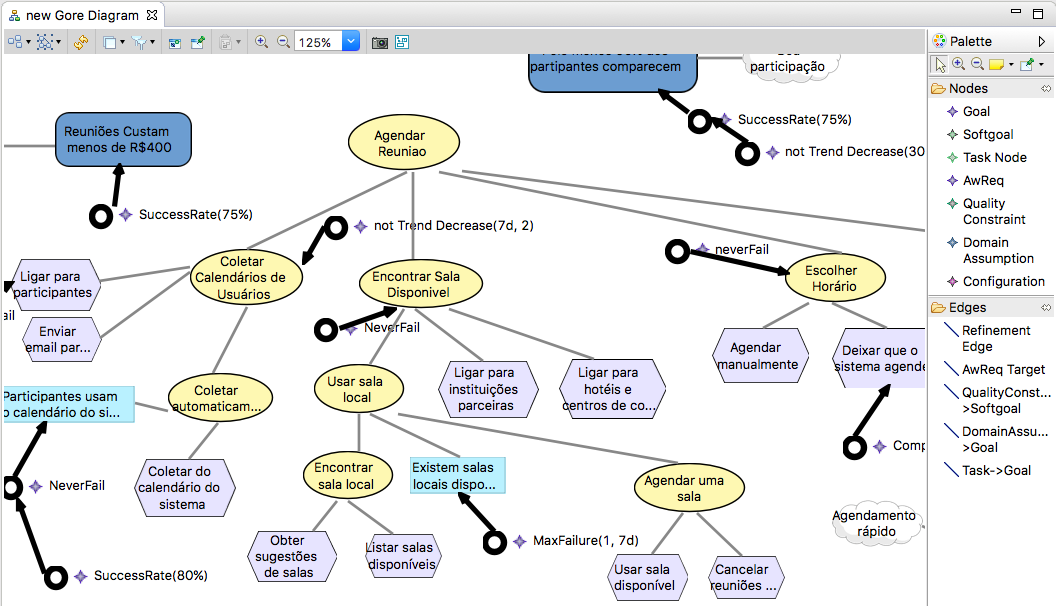
\includegraphics[width=1\textwidth]{figuras/unagi/modeloemunagi.png}
	\caption{Editor Unagi.}
	\label{figura-paleta-unagi}
\end{figure}

\begin{figure}
	\centering
	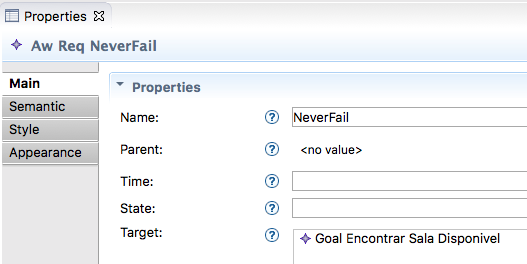
\includegraphics[width=0.85\textwidth]{figuras/unagi/paletaopcoes.png}
	\caption{Editor Unagi - Paleta de Opções.}
	\label{unagi-paleta-opcoes}
\end{figure}

Para acessar a perspectiva que permite o detalhamento dos \evoreqs referentes a cada \awreq é necessário simplesmente um clique duplo sobre o Requisito de Percepção desejado. O editor então oferece a opção de criação de um subdiagrama de detalhamento dos elementos, mostrado na Figura~\ref{figura-subdiagrama-awreq}. Assim, o usuário pode determinar as Condições de Resolução, as Condições de Aplicabilidade e as Estratégias de Adaptação usando a mesma lógica de arrastar e soltar, selecionando os elementos na parte direita da tela. É importante dizer que o modelo só aceita a criação de um elemento específico após seu elemento ``pai'' ter sido criado, por exemplo, só é possível criar uma Estratégia de Adaptação após ter definido uma Condição de Aplicabilidade.

\begin{figure}
	\centering
	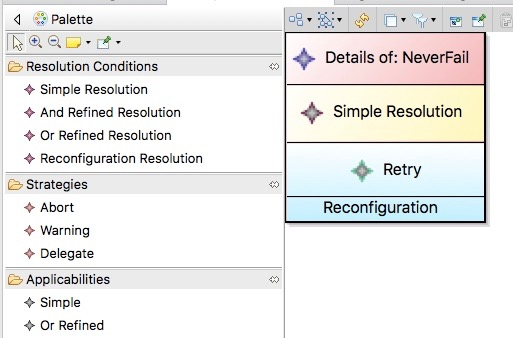
\includegraphics[width=0.85\textwidth]{figuras/unagi/unagisubdiagrama.jpg}
	\caption{Editor Unagi - Subdiagrama de Especificação de \evoreqs.}
	\label{figura-subdiagrama-awreq}
\end{figure}

% ======================================================================================================
% SEÇÃO O Conversor
% ======================================================================================================
\section{Conversor}

\vitor{Faltou esta seção...}

\vitor{Onde pode ser encontrado o código-fonte do Unagi? Antes de você citar a URL do GitHub aqui, acho que deveríamos transferir o repositório para o NEMO. Pode ser?}
% ==============================================================================
% TCC - César Henrique Bernabé
% Capítulo 3 - Projeto Arquitetural e Implementação
% ==============================================================================

\chapter{Validação}
\label{sec-validacao}

Nesse capítulo são discutidas as etapas de verificação e validação de ambos as realizações no contexto desse trabalho: a adaptação do \zanshin a nova proposta de metamodelo e a criação da ferramenta \unagi.

\section{Zanshin}
\label{sec-validacao-zanshin}

O processo de validação do \zanshin teve foco nas simulações de adaptação que já estavam disponíveis. O \framework disponibiliza alguns  exemplos de modelos de sistemas que podem ser usados para simular situações em que  seriam necessárias operações de adaptação sobre os objetivos elicitados. Entre essas simulações disponíveis podemos citar o sistema de agendamento de reuniões (\textit{Meeting Scheduler}) e o sistema de despacho de ambulâncias (\textit{ACAD System}).

Nessa fase, os arquivos \ecore e \xml de especificação dos metamodelos dos sistemas citados foram reescritos para referenciarem corretamente os elementos do novo metamodelo. Primeiramente, o metamodelo anterior referia-se aos refinamentos do objetivo principal como ``children'', e na nova proposta são referenciados como ``refinements'', portanto o primeiro passo foi a modificação do nome da referencia, como mostrado nas listagens~\ref{xml-children} e~\ref{xml-refinements}. 

\begin{lstlisting}[caption={Trecho de XML representando o ACAD no metamodelo antigo},label={xml-children}]
<rootGoal xsi:type="scheduler:G_SchedMeet">
	<children xsi:type="scheduler:T_CharactMeet"/>
		<children xsi:type="scheduler:G_CollectTime" refinementType="or">
			...
		</children>
	...
\end{lstlisting}

\begin{lstlisting}[caption={Trecho de XML representando o ACAD no novo metamodelo},label={xml-refinements}]
<rootGoal xsi:type="scheduler:G_SchedMeet">
	<refinements xsi:type="scheduler:T_CharactMeet">
		<awreqs xsi:type="scheduler:AR1">
			<condition xsi:type="it.unitn.disi.zanshin.model:SimpleResolutionCondition"/>
			<strategies xsi:type="it.unitn.disi.zanshin.model:RetryStrategy" time="5000">
				<condition xsi:type="it.unitn.disi.zanshin.model:MaxExecutionsPerSessionApplicabilityCondition" maxExecutions="2"/>
			</strategies>
		</awreqs>
	</refinements>
	<refinements xsi:type="scheduler:G_CollectTime" refinementType="or">
	...
\end{lstlisting}

Além da substituição do nome para referenciar os refinamentos, pode-se identificar que agora os \awreqs são definidos dentro do escopo do componente ao qual se referem. No processo anterior os \awreqs deviam ser especificados separadamente e conter um campo de referência para o elemento ao qual apontavem, como mostrado na listagem~\ref{xml-awreq-antigo}. A principal vantagem dessa modificação foi o aumento do nível de legibilidade do código do arquivo de especificação já que, como pode ser percebido em~\ref{xml-awreq-antigo}, o alvo do \awreq, definido pela variável ``target'', referenciava a linha a qual o elemento estava descrito. Assim como os refinamentos que deixaram de ser referenciados por ``children'', os \awreqs também passaram a receber uma nova forma de referenciamento: ``awreqs''.
 
\begin{lstlisting}[caption={Trecho de XML representando o ACAD no novo metamodelo},label={xml-refinements}]
	<children xsi:type="scheduler:AR1" target="//@rootGoal/@children.0">
		<condition xsi:type="it.unitn.disi.zanshin.model:SimpleResolutionCondition"/>
		<strategies xsi:type="it.unitn.disi.zanshin.model:RetryStrategy" time="5000">
			<condition xsi:type="it.unitn.disi.zanshin.model:MaxExecutionsPerSessionApplicabilityCondition" maxExecutions="2"/>
		</strategies>
	</children>
\end{lstlisting}

Seguindo a mesma motivação dos elementos anteriores, a referência para \textit{Domain Assumptions} passou de ``children'' para ``assumptions'', caracterizando assim uma separação dos diferentes tipos de refinamentos do modelo, facilitanto então tanto o processo de implementação quando de leitura dos arquivos de especificação. 

Ao final do processo de reescrita dos arquivos dos modelos dos sistemas \textit{Meeting Scheduler} e \textit{ACAD}, ambos foram importados para dentro do \eclipse, onde o \zanshin é executado, e pode-se verificar que o processo de simulação, que não teve nenhuma parte do código modificada, rodou perfeitamente com a nova versão do \zanshin e produziu as saídas esperadas para todos os casos.

Os arquivos completos dos modelos antigos podem ser encontrados no repositório original do \framework~\footnote{https://github.com/sefms-disi-unitn/Zanshin/tree/master/zanshin-simulations/src/it/unitn/disi/zanshin/simulation/cases}, enquanto as novas versões dos mesmos encontram-se em apêndice a esse texto.
% ==============================================================================
% TCC - César Henrique Bernabé
% Capítulo 3 - Considerações Finais
% ==============================================================================
\chapter{Considerações Finais}
\label{sec-conclusoes}

Este capítulo apresenta as conclusões do trabalho realizado, mostrando suas contribuições. Por fim, são apresentadas suas limitações e perspectivas de trabalhos futuros.

\section{Conclusões}
\label{sec-consideracoes-finais-conclusoes}


\section{Limitações e Perspectivas Futuras}
\label{sec-consideracoes-finais-limitacoes-perspectivas}


%%% Páginas finais do documento: bibliografia e anexos. %%%

% Finaliza a parte no bookmark do PDF para que se inicie o bookmark na raiz e adiciona espaço de parte no sumário.
\phantompart

% Marca o início dos elementos pós-textuais.
\postextual

% Referências bibliográficas
\bibliography{bibliografia}


% Apêndices.
\begin{apendicesenv}

% Imprime uma página indicando o início dos apêndices.
\partapendices

% (*) Incluir como apêndice a documentação técnica produzida durante o PG (especificação de requisitos,
% projeto arquitetural, etc.). Utilizar o exemplo \includepdf caso o documento seja produzido em outro
% editor de texto (Microsoft Word, LibreOffice Writer) e transformado em PDF. Utilizar o exemplo \include
% caso os documentos tenham sido também escritos em LaTeX.

%\includepdf[pages={1-}]{apendices/apendice01-documento-requisitos/documento-requisitos.pdf}
%\includepdf[pages={1-}]{apendices/apendice02-documento-projeto/documento-projeto.pdf}

\chapter{Especificação textual do \textit{ACAD}}

\begin{lstlisting}[caption={Especifcação do Sistema ACAD}]
<?xml version="1.0" encoding="UTF-8"?>
	<acad:AcadGoalModel xmi:version="2.0" xmlns:xmi="http://www.omg.org/XMI" xmlns:xsi="http://www.w3.org/2001/XMLSchema-instance" xmlns:ecore="http://www.eclipse.org/emf/2002/Ecore" xmlns:acad="https://raw.githubusercontent.com/hbcesar/zanshin/master/zanshin-simulations/src/it/unitn/disi/zanshin/simulation/cases/acad/acad.ecore" xmlns:eca="https://raw.githubusercontent.com/hbcesar/zanshin/master/it.unitn.disi.zanshin.core/META-INF/eca.ecore">
		<rootGoal xsi:type="acad:G_GenDispatch">
			<refinements xsi:type="acad:G_CallTaking">
				<assumptions xsi:type="acad:D_MaxCalls"/>
				<refinements xsi:type="acad:G_RegCall">
					<refinements xsi:type="acad:T_InputInfo"/>
					<refinements xsi:type="acad:T_DetectLoc"/>
					<awreqs xsi:type="acad:AR15">										
						<condition xsi:type="eca:SimpleResolutionCondition"/>
						<strategies xsi:type="eca:RetryStrategy" time="5000">
							<condition xsi:type="eca:MaxExecutionsPerSessionApplicabilityCondition" maxExecutions="1"/>
						</strategies>
						<strategies xsi:type="eca:RelaxDisableChildStrategy" child="//@rootGoal/@refinements.0/@refinements.0/@refinements.1">
							<condition xsi:type="eca:MaxExecutionsPerSessionApplicabilityCondition" maxExecutions="1"/>
						</strategies>
					</awreqs>
				</refinements>
				<refinements xsi:type="acad:T_ConfirmCall"/>
				<refinements xsi:type="acad:G_AssignIncident">
					<refinements xsi:type="acad:T_SearchDuplic"/>
					<refinements xsi:type="acad:T_CreateOrAssign"/>
				</refinements>
			</refinements>
			<assumptions xsi:type="acad:D_DataUpd"/>
			<refinements xsi:type="acad:G_ResourceId">
				<refinements xsi:type="acad:T_SpecConfig"/>
				<refinements xsi:type="acad:T_ConfIncident"/>
			</refinements>
			<refinements xsi:type="acad:G_ResourceMob">
				<refinements xsi:type="acad:T_DetBestAmb"/>
				<refinements xsi:type="acad:T_InformStat"/>
				<refinements xsi:type="acad:G_RouteAssist" refinementType="or">
					<assumptions xsi:type="acad:D_DriverKnows"/>
					<refinements xsi:type="acad:T_AcadAssists"/>
					<refinements xsi:type="acad:T_StaffAssists"/>
				</refinements>
				<refinements xsi:type="acad:T_Feedback"/>
			</refinements>
			<refinements xsi:type="acad:G_ObtainMap" refinementType="or">
				<assumptions xsi:type="acad:D_GazetUpd"/>
				<refinements xsi:type="acad:G_ManualMap" refinementType="or">
					<refinements xsi:type="acad:T_CheckGazet"/>
					<refinements xsi:type="acad:T_CheckPaper"/>
				</refinements>
			</refinements>
			<refinements xsi:type="acad:G_IncidentUpd">
				<refinements xsi:type="acad:G_MonitorRes">
					<refinements xsi:type="acad:G_UpdPosition" refinementType="or">
						<assumptions xsi:type="acad:D_MDTPos"/>
						<refinements xsi:type="acad:T_RadioPos"/>
					</refinements>
					<assumptions xsi:type="acad:D_MDTUse"/>
					<refinements xsi:type="acad:T_MonitorStatus"/>
					<refinements xsi:type="acad:T_DispStatus"/>
					<refinements xsi:type="acad:T_DispDepArriv"/>
					<refinements xsi:type="acad:G_DispExcept" refinementType="or">
						<refinements xsi:type="acad:T_Except"/>
						<refinements xsi:type="acad:T_ExceptQueue"/>
					</refinements>
				</refinements>
				<refinements xsi:type="acad:T_CloseIncident"/>
				<refinements xsi:type="acad:T_ReplAmb"/>
			</refinements>

			<!-- Softgoals. -->
			<refinements xsi:type="acad:S_FastArriv">
				<constraints xsi:type="acad:Q_AmbArriv"/>
			</refinements>
			<refinements xsi:type="acad:S_FastDispatch">
				<constraints xsi:type="acad:Q_Dispatch">
					<awreqs xsi:type="acad:AR11" incrementCoefficient="2">						
						<condition xsi:type="eca:ReconfigurationResolutionCondition"/>
						<strategies xsi:type="eca:ReconfigurationStrategy" algorithmId="qualia">
							<condition xsi:type="eca:ReconfigurationApplicabilityCondition"/>
						</strategies>
					</awreqs>
				</constraints>
			</refinements>
			<refinements xsi:type="acad:S_FastAssist">
				<constraints xsi:type="acad:Q_IncidResolv"/>
			</refinements>
			<refinements xsi:type="acad:S_LowCost">
				<constraints xsi:type="acad:Q_MaxCost"/>
			</refinements>
			<refinements xsi:type="acad:S_UserFriendly">
				<constraints xsi:type="acad:Q_MaxTimeMsg"/>
			</refinements>
	</rootGoal>

	<!-- System parameters. -->
	<configuration>
		<parameters xsi:type="acad:CV_MST" type="ncv" unit="10" value="60" metric="integer"/>
	</configuration>

	<!-- Indicator / parameter differential relations. -->
	<relations indicator="//@rootGoal/@refinements.6/@constraints.0/@awreqs.0" parameter="//@configuration/@parameters.0" lowerBound="0" upperBound="180" operator="ft" />
</acad:AcadGoalModel>

\end{lstlisting}
\chapter{Especificação textual do \textit{Meeting Scheduler}}

\begin{lstlisting}[caption={Especifcação do Sistema Meeting Scheduler}]
<?xml version="1.0" encoding="UTF-8"?>
<scheduler:SchedulerGoalModel xmi:version="2.0" xmlns:xmi="http://www.omg.org/XMI" xmlns:xsi="http://www.w3.org/2001/XMLSchema-instance" xmlns:scheduler="https://raw.githubusercontent.com/hbcesar/zanshin/master/zanshin-simulations/src/it/unitn/disi/zanshin/simulation/cases/scheduler/scheduler.ecore" xmlns:it.unitn.disi.zanshin.model="https://raw.githubusercontent.com/hbcesar/zanshin/master/it.unitn.disi.zanshin.core/META-INF/eca.ecore">
	<rootGoal xsi:type="scheduler:G_SchedMeet">
		<refinements xsi:type="scheduler:T_CharactMeet">
			<awreqs xsi:type="scheduler:AR1">
				<condition xsi:type="it.unitn.disi.zanshin.model:SimpleResolutionCondition"/>
				<strategies xsi:type="it.unitn.disi.zanshin.model:RetryStrategy" time="5000">
					<condition xsi:type="it.unitn.disi.zanshin.model:MaxExecutionsPerSessionApplicabilityCondition" maxExecutions="2"/>
				</strategies>
			</awreqs>
		</refinements>
		<refinements xsi:type="scheduler:G_CollectTime" refinementType="or">
			<refinements xsi:type="scheduler:T_CallPartic"/>
			<refinements xsi:type="scheduler:T_EmailPartic"/>
			<refinements xsi:type="scheduler:G_CollectAuto">
				<assumptions xsi:type="scheduler:D_ParticUseCal"/>
				<refinements xsi:type="scheduler:T_CollectCal"/>
			</refinements>
		</refinements>
		<refinements xsi:type="scheduler:G_FindRoom" refinementType="or">
			<refinements xsi:type="scheduler:G_UseLocal">
				<refinements xsi:type="scheduler:G_FindLocal" refinementType="or">
					<refinements xsi:type="scheduler:T_GetSuggest"/>
					<refinements xsi:type="scheduler:T_ListAvail"/>
				</refinements>
				<assumptions xsi:type="scheduler:D_LocalAvail"/>
				<refinements xsi:type="scheduler:G_BookRoom" refinementType="or">
					<refinements xsi:type="scheduler:T_UseAvail"/>
					<refinements xsi:type="scheduler:T_CancelLess"/>
				</refinements>
			</refinements>
			<refinements xsi:type="scheduler:T_CallPartner"/>
			<refinements xsi:type="scheduler:T_CallHotel"/>
			<awreqs xsi:type="scheduler:AR4">
				<condition xsi:type="it.unitn.disi.zanshin.model:ReconfigurationResolutionCondition"/>
				<strategies xsi:type="it.unitn.disi.zanshin.model:ReconfigurationStrategy" algorithmId="qualia">
					<condition xsi:type="it.unitn.disi.zanshin.model:ReconfigurationApplicabilityCondition"/>
				</strategies>
			</awreqs>
		</refinements>
		<refinements xsi:type="scheduler:G_ChooseSched" refinementType="or">
			<refinements xsi:type="scheduler:T_SchedManual"/>
			<refinements xsi:type="scheduler:T_SchedSystem"/>
		</refinements>
		<refinements xsi:type="scheduler:G_ManageMeet" refinementType="or">
			<refinements xsi:type="scheduler:T_CancelMeet"/>
			<refinements xsi:type="scheduler:T_CancelMeet"/>
		</refinements>
		<refinements xsi:type="scheduler:S_LowCost">
			<constraints xsi:type="scheduler:Q_CostLess100"/>
		</refinements>
		<refinements xsi:type="scheduler:S_GoodPartic">
			<constraints xsi:type="scheduler:Q_Min90pctPart"/>
		</refinements>
		<refinements xsi:type="scheduler:S_FastSched">
			<constraints xsi:type="scheduler:Q_Sched1Day"/>
		</refinements> 
	</rootGoal>
	
	<configuration>
		<parameters xsi:type="scheduler:CV_RfM" unit="1" value="5" metric="integer"/>
	</configuration>
	
	<relations indicator="//@rootGoal/@refinements.0/@awreqs.0" parameter="//@configuration/@parameters.0" lowerBound="0" upperBound="10"/>
</scheduler:SchedulerGoalModel>

\end{lstlisting}
\end{apendicesenv}


% Índice remissivo.
\phantompart
\printindex

% Fim do documento.
\end{document}
